\documentclass[proof,pdftex,11pt,a4,titlepage]{article}
\usepackage[parfill]{parskip}
\usepackage{lmodern}
\usepackage{amsmath, amsthm, amssymb}
\usepackage[usenames,dvipsnames]{xcolor}
\usepackage{tikz}
\usepackage{subcaption}
\usepackage{placeins}
\usepackage[pdftex]{graphicx}
\usepackage[T1]{fontenc}
\usepackage[utf8]{inputenc}
\usepackage{calc}
\usepackage{tabularx}
\usepackage{multirow}
\usepackage{rotating}
\usepackage{proof}
\usepackage{appendix}
\usepackage{breqn}

\usepackage{afterpage}
\newcommand\blankpage{%
    \null
    \thispagestyle{empty}%
    \addtocounter{page}{-1}%
    \newpage}

\usepackage{pgfplots}

\usepackage{graphicx}
\DeclareGraphicsExtensions{.png}

\newcommand{\credit}[1]{\par\hfill \footnotesize Credit: #1}

\usepackage{listings}
\usepackage{inconsolata}
\lstset{basicstyle=\footnotesize\ttfamily,breaklines=true}
\lstset{language=Python, basewidth=0.5em,
  keywordstyle=\color{blue}, commentstyle=\color{Green}, stringstyle=\color{Red}}

\def\code{\lstinline[basicstyle=\textsize\ttfamily]}

\newcommand{\sat}{\textsc{sat}}
\newcommand{\unsat}{\textsc{unsat}}

\begin{document}

\title{\textbf{Exploring Strategies for Performing Extended Resolution as a Preprocessing Step for SAT-Solving}}
\author{Eliot Ball}

\maketitle

\blankpage

\thispagestyle{empty}

\section*{Summary}

Prior research in the field of logic has shown that the \emph{extended resolution} proof system can facilitate polynomial-length proofs of propositions that require exponential-length proofs in the \emph{resolution} proof system. Based on this, some research has been carried out within the field of software and hardware verification into using extended resolution as a part the procedure followed by a \sat{}-solver, with varying success. I explore, through the use of \emph{genetic algorithms}, whether extension can be used effectively as a preprocessing step that removes redundancy prior to running a \sat{}-solver. Because of their important practical applications, I focus on formulas obtained from software verification problems.

\tableofcontents

\newpage
\blankpage

\setcounter{page}{1}
\section{Introduction}

In a world increasingly driven by machines and other automated systems, bugs and mistakes made by the creators of these machines are expensive, and sometimes dangerous. In 1994, Intel was pressured into replacing a huge batch of its Pentium processors when it was discovered that the floating point unit within them was faulty, often returning inaccurate results. This recall cost Intel \$475 million \cite{Nicely:2008}. This type of mistake is often a huge problem for the parties involved, and it is easy to imagine truly disastrous outcomes if a mistake is made in the software for a missile guidance system, or the control systems for a car.

This raises the question of how to be sure that a system is correct --- answering the question, ``have we implemented what we intended to implement?'' Testing a system, by trying out all of the different types of situations we think it can reach, can only go so far. What if we fail to foresee some of the situations? Ideally, we would be able to prove beyond doubt that the system does not fail.

There are several approaches to this, each with their own strengths and weaknesses \cite{Dsilva:2008}. Bounded Model Checking (BMC) is one approach, where a system is encoded as a propositional formula that can be thought of as expressing the claim ``There is a counterexample, proving this system flawed, of length at most $k$'', for some given $k$ \cite{Biere:1999}. This formula is then checked to see whether it is satisfiable using a \sat{}-solver. If the formula is satisfiable, then there is a counterexample of the desired length, which may be obtained by inspecting the values of the variables in a satisfying assignment. If the formula is not satisfiable, then we can be sure that there is not a counterexample of the desired length. The smallest possible $k$ guaranteeing that the system is completely correct (that there is no counterexample of any length) is called the \emph{completeness threshold} \cite{Kroening:2003}. In general, finding the completeness threshold is as hard as actually verifying the system, but many errors are shallow, and may be found with a low value of $k$. Therefore, using even a fairly small value can increase one's confidence in a system, even if one can still not be \emph{completely sure} that the system is correct. Since this approach involes generating a formula for a \sat{}-solver, the efficiency of any BMC tool is tied to the performance of current \sat{}-solvers. \sat{}-solvers have become increasingly efficient over recent years (see Figure \ref{fig:sat-solver-perf}), and BMC has therefore become more and more effective for model verification.

\begin{figure}[h]
  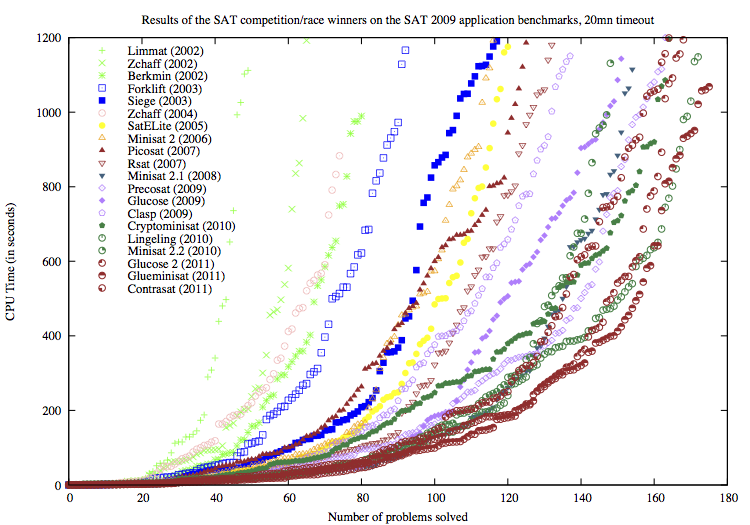
\includegraphics[width=\textwidth]{sat-perf}
  \credit{Daniel Le Berre}
  \caption{The increasing performance of modern \sat{}-solvers.}
  \label{fig:sat-solver-perf}
\end{figure}

For a given proposition about a system, there are multiple ways of encoding that proposition as a propositional formula, and the encoding we choose can affect the performance of a \sat{}-solver on that formula. For example, the naive method for encoding ``at-most-one'' constrains (that is, constraints of the form $x_1 + x_2+ \cdots + x_n \leq k$ where $x_i \in \{0,1\}$) produces large formulas that lead to bad performance for \sat{}-solvers. A more intelligent approach to encoding leads to much better performance (See Section \ref{sec:encoding} for more details).

Given that choice of encoding can have a significant effect on both the complexity of the formula produced, and on the subsequent performance of a \sat{}-solver on that formula, it is natural to attempt to preprocess a formula before running a \sat{}-solver, an an attempt to shrink the formula or otherwise mould it more to the specific abilities of the solver.

\section{Boolean satisfiability}

[More definitions]

Modern \sat{}-solvers operate on a machine-readable representation of formulas in \emph{conjunctive normal form} (CNF). For every propositional formula, there is an equivalent CNF formula, which can be found by repeated application of DeMorgan's laws, and the laws about distributivity and double negatives \cite{Plaisted:1986}. Therefore \sat{}-solvers can effectively operate on all propositional formulas.

We define a CNF formula as a conjunction of clauses, where each clause is a disjunction of literals:
\[(l_1 \vee l_2 \vee \cdots \vee l_j) \wedge (l_{j+1} \vee l_{j+2} \vee \cdots \vee l_k) \wedge \cdots \wedge (l_{m+1} \vee l_{m+2} \vee \cdots \vee l_n)\]
Each literal is either a variable or its negation. Note that this formula just requires one literal from each clause to be true.

\subsection{CDCL SAT-solvers}

The most efficient modern \sat{}-solvers operate according to versions of the Davis-Putnam-Logemann-Loveland (DPLL) algorithm. The basis of this algorithm is essentially a depth-first search with backtracking of the whole space of partial assignments, looking for a full assignment that satisfies the formula. In the worst case, this type of exhaustive search would take $O(2^n)$ time to complete for a formula of $n$ variables. \sat{}-solvers can achieve much better performance in practice through the use of a number of heuristics. The DPLL algorithm introduced \emph{unit propagation}, which is the immediate assignment of the required value to any variables found on their own in a clause, and \emph{pure literal elimination}, which is the immediate assignment to any variable which is only found in one polarity in the whole formula (thereby making every clause containing that variable true) \cite{Davis:1962}. The latest \sat{}-solvers, such as \textsc{MiniSat}, heavily exploit further optimisations such as faster data structures for the backtracking algorithm, better strategies for picking which variable to set at each step, and more advanced strategies for backtracking when a conflict is found \cite{Een:2003}. In particular, \emph{conflict driven clause learning} (CDCL) aims to infer a clause from a conflict which encapsulates, in some sense, the `reason' for the conflict, and causes the backtracking algorithm to fail more quickly on other paths that would lead to failure for the same reason.

\subsection{Encodings and preprocessing}
\label{sec:encoding}

The choice of encoding can dramatically affect the size of a formula representing some proposition about a system. Let $x_1, x_2, \ldots, x_n \in \{0, 1\}$, and consider propositions of the form
\[x_1 + x_2 + \cdots + x_n \leq k.\]
A naive encoding of this constraint requires ${n \choose k+1}$ clauses. For example, let $x_1, \ldots, x_4$ be boolean variables, and require that
\[x_1 + x_2 + x_3 + x_4 \leq 1.\]
For a naive encoding of this proposition, it is sufficient that each pair of variables include one that is false, since that will entail that at most one variable is true in the whole set, which satisfies the requirement above. This encoding produces
\begin{align*}
  (\neg x_1 \vee \neg x_2) & \wedge (\neg x_1 \vee \neg x_3) \wedge (\neg x_1 \vee \neg x_4) \\
  & \wedge (\neg x_2 \vee \neg x_3) \wedge (\neg x_2 \vee \neg x_4) \wedge (\neg x_3 \vee \neg x_4).
\end{align*}
Even in this case, where $k=1$, $O(n^2)$ clauses are required. There are, however, a number of approaches to encoding these constraints that lead to much smaller formulas \cite{Biere:2014}. For example, the formula above can be encoded by first arranging the four variables in a matrix:

\begin{center}
  \begin{tabular}{c|cc}
      & 1 & 2 \\ \hline
    1 & $x_1$ & $x_2$ \\
    2 & $x_3$ & $x_4$
  \end{tabular}
\end{center}

Then we introduce a variable $c_n$ for each column $n$, and a variable $r_m$ for each row $m$. We then add two clauses for each variable $x_i$. If $x_i$ is in column $n$ and row $m$, we add
\begin{align*}
  x_i \to c_n &= \neg x_i \vee c_n, \\
  x_i \to r_m &= \neg x_i \vee r_m.
\end{align*}
In the above case, we add $(\neg x_3 \vee c_1) \wedge (\neg x_3 \vee r_2)$ for the $x_3$ variable, for example.

These clauses mean that any of the variables in column $n$ being true will cause $c_n$ to be true, and any of the variables in row $m$ being true will cause $r_m$ to be true. Then, we simply require that at most one column, and at most one row contains a true variable, so
\[(\neg c_1 \vee \neg c_2) \wedge (\neg r_1 \vee \neg r_2).\]
It is possible to arrange $n$ variables in a $p$ by $q$ matrix where $p = \lfloor \sqrt{n} \rfloor = O(\sqrt{n})$ and $q = \lceil n / p \rceil = O(\sqrt{n})$. Therefore, to encode the formula with this approach, we need $O(n)$ clauses specifying the location of each variable, $O(p^2)=O(n)$ clauses ensuring that only one row contains a true variable, and $O(q^2)=O(n)$ clauses ensuring that only one column contains a true variable. Therefore this encoding requires only $O(n)$ clauses in total, a huge (asymptotic\footnote{The encoding is better in absolute terms when $n>47$ \cite{Biere:2014}.}) improvement over the $O(n^2)$ clauses required by the naive encoding.

[Work below here]

The problem of picking an encoding for a proposition suggests the idea of pre-processing a formula before the \sat{}-solver is run. It may be possible to detect opportunities to re-structure a formula in such a way that the \sat{}-solver returns the result in less time. If the time saved by the \sat{}-solver is greater than the time taken to detect and apply the optimisations, then a net gain is made.

[More from Ruben still to incorporate]

\section{Resolution and extended resolution}

The \emph{pigeonhole principle} states that, if $n > m$, it is impossible to place $n$ items in $m$ bins without any bins containing more than one item. We can attempt to verify this by encoding the contrapositive, ``it is possible to place $n>m$ items in $m$ bins without any bin containing more than one item'' as a propositional formula, and then showing that it is \unsat. As $n$ could be arbitrarily larger than $m$, we will actually show that the propositional formula encoding the assertion ``it is possible to place $n$ items in $n-1$ bins without any bin containing more than one item'' is \unsat. If it is impossible to place $n$ items in $n-1$ bins in this way, then it is certainly impossible to place even more than $n$ items (since we have to place $n$ items in $n-1$ bins on the way), so this assertion suffices.

Let $P_{i,b}$ be a propositional variable standing for item $i$ being placed in bin $b$. Then we start by asserting that, for all items $1 \leq i \leq n$,
\[P_{i,1} \vee P_{i,2} \vee \cdots \vee P_{i,n-1}.\]
That is, for every item, it's either in bin 1, bin 2, \dots, or bin $n-1$ --- so every item is in a bin. Then we assert that, for every bin $1 \leq b \leq n-1$, for each pair of items $1 \leq i < j \leq n$,
\[\neg P_{i,b} \vee \neg P_{j,b}.\]
That is, for each bin, for each pair of items, one or other of those items is not in the bin --- so no pair of items is in the same bin. Together, these clauses assert that it is possible to place $n$ items in $n-1$ bins without more than one item in any bin. This formula is \unsat.

One way of proving that this formula is \unsat{} is to provide a resolution refutation. Where clauses are respresented as sets of literals (e.g. $a \vee \neg b$ is represented by $\{a, \neg b\}$), the resolution rule works as follows.\[
\infer[\mathrm{res}]{C_1 \cup C_2}{
  C_1 \cup \{L\}
  &
  C_2 \cup \{\neg L\}
}
\]

For example, we can use resolution to prove the pigeonhole principle for the easy $n = 2$ case (where there is only one bin):\[
\infer[\mathrm{res}]{\bot}{
  \infer[\mathrm{res}]{\{\neg P_{2,1}\}}{
    \{P_{1,1}\}
    &
    \{\neg P_{1,1}, \neg P_{2,1}\}
  }
  &
  \{P_{2,1}\}
}
\]

This is, in fact, a \emph{tree resolution} proof, because no clause is an antecedent of more than one other clause. Unfortunately, for sufficiently large $n$, a tree resolution proof of the pigeonhole principle for $n$ items requires $2^{\Omega(n)}$ steps, suggesting that tree resolution may not be the best proof system with which to prove the pigeonhole principle \cite{Haken:1985}.
However, runs of DPLL-based \sat{}-solvers on \unsat{} formulas correspond to tree resolution refutations of the formula, which suggests that such \sat{}-solvers will exhibit low performance on instances of the pigeonhole principle, and perhaps other similar formulas \cite{Rossi:2006}. This raises the question of whether there is a more powerful system that allows a sub-exponential length proof -- and thus better performance by a DPLL-based \sat{}-solver -- on this type of instance. These systems do exist, and one such system is \emph{extended resolution}.

Extended resolution adds an additional rule beyond the resolution rule. Given a pair of literals $l_1$ and $l_2$ from the propositional formula, and a fresh variable $x$, we may introduce a new set of clauses representing $x \leftrightarrow l_1 \vee l_2$ \cite{Tseitin:1983}. The set of clauses representing this addition is

\begin{equation*}
  \begin{align*}
    x \leftrightarrow l_1 \vee l_2 &= (x \to (l_1 \vee l_2)) \wedge (l_1 \to x) \wedge (l_2 \to x) \\
          &= (\neg x \vee l_1 \vee l_2) \wedge (\neg l_1 \vee x) \wedge (\neg l_2 \vee x).
  \end{align*}
\end{equation*}

Extended resolution permits a polynomial-length proof of the pigeonhole principle \cite{Cook:1976}, which is outlined below.

A conventional proof of the pigeonhole principle works by induction on $n$. First, it can easily be shown that it's not possible to assign 2 items to 1 bin without the sole bin containing more than one item (it will have to contain both!), as we did by resolution above. We will see this as the lack of an injective mapping from $\{1,2\}$ to $\{1\}$. Then, for the inductive step, we show that if there is a mapping from $\{1,2,\ldots,n\}$ to $\{1,2,\ldots,n-1\}$, then there is a mapping from $\{1,2,\ldots,n-1\}$ to $\{1,2,\ldots,n-2\}$. We do this by supposing that $\phi$ is an injective mapping from $\{1,2,\ldots,n\}$ to $\{1,2,\ldots,n-1\}$, in which case
\[\phi'(i) = \begin{cases}
\phi(n) & \mbox{if } \phi(i) = n-1, \\
\phi(i) & \mbox{otherwise}
\end{cases}\]
is an injective mapping from $\{1,2,\ldots,n-1\}$ to $\{1,2,\ldots,n-2\}$. Intuitively, $\phi'$ maps everything in the same way as $\phi$, except that the mappings \emph{from} $n$ and \emph{to} $n-1$ are merged, allowing those numbers to be deleted (see Figure \ref{fig:php-induction}). Since there isn't a mapping for $n=2$, by contradiction there can't be one for $n=3$, and therefore there is none for $n=4$, and so on.

\begin{figure}[h]
  \begin{subfigure}[H]{0.5\textwidth}
    \centering
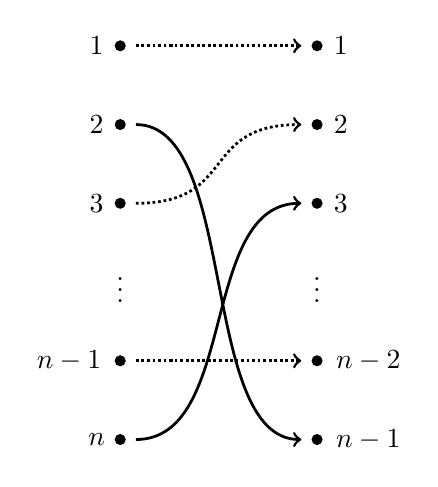
\begin{tikzpicture}
\fill (1,5) circle (2pt);
\fill (1,4) circle (2pt);
\fill (1,3) circle (2pt);
\fill (1,1) circle (2pt);
\fill (1,0) circle (2pt);

\fill (3.5,5) circle (2pt);
\fill (3.5,4) circle (2pt);
\fill (3.5,3) circle (2pt);
\fill (3.5,1) circle (2pt);
\fill (3.5,0) circle (2pt);

\node[draw=none] at (1,2) {$\vdots$};
\node[draw=none] at (3.5,2) {$\vdots$};

\node[draw=none] at (0.7,5) {1};
\node[draw=none] at (0.7,4) {2};
\node[draw=none] at (0.7,3) {3};
\node[draw=none] at (0.35,1) {$n-1$};
\node[draw=none] at (0.7,0) {$n$};

\node[draw=none] at (3.8,5) {1};
\node[draw=none] at (3.8,4) {2};
\node[draw=none] at (3.8,3) {3};
\node[draw=none] at (4.15,1) {$n-2$};
\node[draw=none] at (4.15,0) {$n-1$};

\draw[line width=1pt, densely dotted] [->] (1.2,5) .. controls (2.5,5) and (2,5) .. (3.3,5);
\draw[line width=1pt] [->] (1.2,4) .. controls (2.5,4) and (2,0) .. (3.3,0);
\draw[line width=1pt, densely dotted] [->] (1.2,3) .. controls (2.5,3) and (2,4) .. (3.3,4);
\draw[line width=1pt, densely dotted] [->] (1.2,1) .. controls (2.5,1) and (2,1) .. (3.3,1);
\draw[line width=1pt] [->] (1.2,0) .. controls (2.5,0) and (2,3) .. (3.3,3);
\end{tikzpicture}

    \caption{An example mapping $\phi$}
  \end{subfigure}
  %
  \begin{subfigure}[H]{0.5\textwidth}
    \centering
\begin{tikzpicture}
\fill (1,5) circle (2pt);
\fill (1,4) circle (2pt);
\fill (1,3) circle (2pt);
\fill (1,1) circle (2pt);

% offset hack
\fill[color=white] (1,0) circle (2pt);
\node[draw=none, color=white] at (1,0) {0};

\fill (3.5,5) circle (2pt);
\fill (3.5,4) circle (2pt);
\fill (3.5,3) circle (2pt);
\fill (3.5,1) circle (2pt);

\node[draw=none] at (1,2) {$\vdots$};
\node[draw=none] at (3.5,2) {$\vdots$};

\node[draw=none] at (0.7,5) {1};
\node[draw=none] at (0.7,4) {2};
\node[draw=none] at (0.7,3) {3};
\node[draw=none] at (0.35,1) {$n-1$};

\node[draw=none] at (3.8,5) {1};
\node[draw=none] at (3.8,4) {2};
\node[draw=none] at (3.8,3) {3};
\node[draw=none] at (4.15,1) {$n-2$};

\draw[line width=1pt, densely dotted] [->] (1.2,5) .. controls (2.5,5) and (2,5) .. (3.3,5);
\draw[line width=1pt] [->] (1.2,4) .. controls (2.5,4) and (2,3) .. (3.3,3);
\draw[line width=1pt, densely dotted] [->] (1.2,3) .. controls (2.5,3) and (2,4) .. (3.3,4);
\draw[line width=1pt, densely dotted] [->] (1.2,1) .. controls (2.5,1) and (2,1) .. (3.3,1);
\end{tikzpicture}

    \caption{The derived $\phi'$}
  \end{subfigure}
  \caption{An illustration of the inductive step in proving the pigeonhole principle.}
  \label{fig:php-induction}
\end{figure}

The extended resolution proof mirrors this process. Suppose we have the clauses restricting the values of $P_{i,b}$ for some instance of the pigeonhole principle, as given above. These clauses, if they are satisfiable, imply some mapping $\phi$. We now introduce new propositional variables $Q_{i,b}$, with $1 \leq i \leq n-1$ and $1 \leq b \leq n-2$, which, if satisfiable, describe the corresponding mapping $\phi'$. We set

\begin{equation*}
  \begin{align*}
    Q_{i,b} &= P_{i,b} \vee (P_{i,n-1} \wedge P_{n,b}) \\
      &= (P_{i,b} \vee P_{i,n-1}) \wedge (P_{i,b} \vee P_{n,b}),
  \end{align*}
\end{equation*}

which just says that the new mapping of a particular item ($Q_{i,b}$) either matches the old one ($P_{i,b}$) or it represents that merge between the mappings from $n$ and to $n-1$ ($P_{i,n-1} \wedge P_{n,b}$). This can be achieved by performing two extensions per variable $Q_{i,b}$:

\begin{equation*}
  \begin{align*}
    Q_{i,b} &\leftrightarrow P_{i,b} \vee P_{i,n-1} \\
    Q_{i,b} &\leftrightarrow P_{i,b} \vee P_{n,b}
  \end{align*}
\end{equation*}

From this new (polynomial-size) set of clauses, and the clauses given by the instance of the pigeonhole principle for $n$ items, we can obtain, by a polynomial number of resolutions, the following clauses:

\begin{table}[h]
  \begin{tabular}{rll}
        & $Q_{i,1} \vee Q_{i,2} \vee \cdots \vee Q_{i,n-2}$ & for $1 \leq i \leq n-1$, \\
    and & $\neg Q_{i,b} \vee \neg Q_{j,b}$ & for $1 \leq b \leq n-2$ and $1 \leq i < j \leq n-1$.
  \end{tabular}
\end{table}
\FloatBarrier

(See Appendix A for a worked example.) These clauses describe the pigeonhole principle for $n-1$ items. Repeating this process of extension and resolution $O(n)$ times, until we reach the $n=2$ case, gives a polynomial-length proof of the pigeonhole principle.

\section{Strategies for extension}

We have seen by the example of the pigeonhole principle that adding extension to the resolution proof system can sometimes permit polynomial-length proofs of assertions that would otherwise require exponential length. Since tree resolution proofs correspond to runs of DPLL-based \sat{}-solvers, adding the ability to perform extension in the process of \sat{}-solving can potentially improve the performance of \sat{}-solvers.

In 2010, a restriction of extended resolution was demonstrated which may be used to create a \sat{}-solver that, in some cases, outperforms ones that do not use extension \cite{Audemard:2010}. The authors note that, prior to their paper, no \sat{}-solver based on extended resolution had been proposed, because ``it is hard to devise a heuristic that introduces variables that are likely to help find a short refutation''. In other words, it is unclear which extensions to perform, in order to increase performance. They propose restricting the situations where extension may be performed to those where there are two clauses, $C_1 = l_1 \vee \alpha$ and $C_2 = l_2 \vee \beta$, where neither $\alpha$ nor $\beta$ contain negations of any literals contained in the other, in which case extension may be performed to introduce $z \leftrightarrow \neg l_1 \vee \neg l_2$. The aim of doing so is to avoid redundancy in any later sequence of resolutions producing a new pair of clauses which essentially only differ in that one includes $l_1$ and the other $l_2$. They describe a performant way of implementing this strategy that outperformed state-of-the-art \sat{}-solvers on instances from recent competitions.

In 2015, a group of students explored the possibility of using \emph{common subexpression elimination} (CSE) in various ways to improve the performance of \sat{}-solving \cite{Yan:2015}. They suggest eliminating certain repeated subexpressions by introducing new variables using a generalised version of extension (although they do not actually mention extended resolution themselves). If $\{l_1, l_2, \ldots, l_n\}$ is a set of literals from a propositional formula and $x$ is a fresh variable, then we can introduce the clauses necessary to establish
\[x \leftrightarrow l_1 \vee l_2 \vee \cdots \vee l_n\]
and then, in any clause containing all of $l_1, l_2, \ldots, l_n$, delete those literals, and add $x$. Three methods are given for choosing which subexpressions to eliminate. In the first, the common subexpressions are chosen such that, after they are eliminated, the problem is of minimal size. The authors conjecture that this problem is NP-hard, and give two approximate algorithms. One is based on replacing subexpressions that are found with frequency above a given threshold, and the other is based on the LZW string-compression algorithm. All of these strategies are implemented as a pre-processing step before running the \sat{}-solver. This approach is attractive because of its simplicity, and the authors find an improvement in performance in about half the cases they try.

[Need to motivate this much more --- see Ruben's notes]

For this project, I hypothesise that, for some propositional formulas arising in real-world model checking, there are sets of substitutions of repeated subclauses with size 2 or 3 (that is, there are pairs or triplets of literals which appear in multiple clauses) which can be replaced by extension with a single variable, leading to an improvement in the performance of the \textsc{MiniSat} solver on those instances. I investigate this by attempting to use a genetic algorithm to find such sets of substitutions.

\section{Genetic algorithms}

A \emph{genetic algorithm} is a search algorithm that mimics natural selection. In the most basic form of the algorithm, sufficiently long binary strings are mapped onto the search space, and then an initial population of random strings is created. Each of the strings is scored according to the fitness of the corresponding item in the search space, and then a sample of the most highly-scored strings is taken. From this sample, a new population the same size as the original is created, by taking random pairs of strings from the sample and combining them in a specific way (see below). This process of scoring, sampling, and combining is repeated a nubmer of times, in the hope of finding a member of the search space with high fitness.

In the step where a new population is being generated from the high-fitness sample, the new population members are usually generated according to the following algorithm (See Figure \ref{fig:genetic-algo}):

\begin{enumerate}
  \item {\bf Selection:} Randomly choose two \emph{parents} $a$ and $b$ from the high-fitness sample.
  \item {\bf Crossover:} Where $n$ is the length of the strings, pick some integer $k$ such that $0 \leq k \leq n$, and then combine the two parent strings to create the new member $m = a[0 \ldots k) \parallel b[k \ldots n)$.
  \item {\bf Mutation:} Randomly flip some of the bits in $m$ and then add it to the new population.
\end{enumerate}

\begin{figure}[h]
  \centering
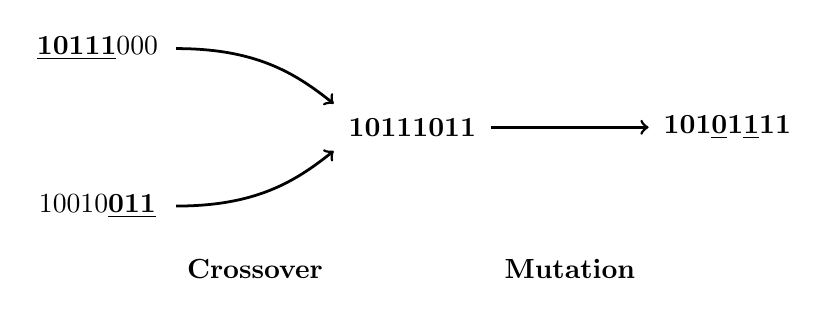
\begin{tikzpicture}
  \node[draw=none] at (0,1) {10010\underline{\bf 011}};
  \node[draw=none] at (0,3) {\underline{\bf 10111}000};

  \node[draw=none] at (4,2) {\bf 10111011};
  \node[draw=none] at (2,0.2) {\bf Crossover};

  \node[draw=none] at (8,2) {\bf 101\underline{0}1\underline{1}11};
  \node[draw=none] at (6,0.2) {\bf Mutation};

  \draw[line width=1pt] [->] (1.0,3) .. controls (2.0,3.0) and (2.5,2.7) .. (3.0,2.3);
  \draw[line width=1pt] [->] (1.0,1) .. controls (2.0,1.0) and (2.5,1.3) .. (3.0,1.7);
  \draw[line width=1pt] [->] (5.0,2) to (7.0,2);
\end{tikzpicture}

  \caption{An illustration of the generation of a new member from a pair of parents in a genetic algorithm.}
  \label{fig:genetic-algo}
\end{figure}

The aim of the crossover part of the algorithm is to allow good features that are developed in separate members of the population to be combined as ``building blocks'', sometimes leading to a member of the population that is stronger than either of the original members \cite{Goldberg:1989}. In some variations on the basic genetic algorithm, multiple ``cuts'' are made so that more than two members of the population may be combined, but this hasn't been found to produce better final outcomes in most cases, and can lead to premature convergence, owing to a loss of genetic diversity in the population \cite{Esquivel:1997}.

The aim of the mutation part of the algorithm is to allow the exploration of ``nearby'' members of the population. If the search space is sufficiently smooth with respect to the fitness function, then this leads to a hillclimbing effect. This also means that care must be taken with the encoding of solutions as bit vectors, and when setting the rate of mutation, since certain encodings or rates of mutation may not lead to a sufficiently similar ``neighbouring'' solutions for the hillclimbing effect to work correctly \cite{Taher:2013}. In general, the probability of any bit in a member of the population being flipped should not be above 0.05, and with a mutation rate below that threshold, the population size should be between approximately 30 and 100 \cite{Grefenstette:1986}.

There are several different strategies for the selection phase, where the high-fitness sample is chosen \cite{Thierens:1994}. The simplest is \emph{truncation selection}, which is the outcome of sorting the population by fitness, and taking the best $k$ members, for some $k$. An alternative approach is \emph{fitness proportionate selection}, also called \emph{roulette-wheel selection}, where we calculate the fitness of each individual, and then assign each individual some part of the $[0,1]$ interval, so that the size of each individual's section of the interval is proportional to its fitness. Then a random point in the $[0,1]$ interval is picked, and the corresponding member of the population is added to the high-fitness sample. This is repeated $k$ times, where $k$ is the desired size of the high-fitness sample. Both of these strategies generally perform well, but fitness proportionate selection can run in to problems at later stages of execution when the fitness values of the population are similar, as it might not provide enough selection pressure to improve the population \cite{Whitley:1989}. As the fitness values of members of the population in this project are indeed likely to be similar, I chose to use truncation selection.

% Elitism

\section{Technical implementation}

In the technical implementation of this project, I obtained a number of benchmarks that come from real-world bounded model checking. The benchmarks come from implementations of the Newton-Raphson method, polynomial approximations of sine, and squaring of floating-point numbers. To execute the genetic algorithm on a given benchmark, we follow this algorithm:

\begin{samepage}
  \begin{enumerate}
    \item Find, and number, all of the repeated subclauses of size 2 or 3.
    \item Generate an initial population of 50 bit vectors, each having one bit per subclause.
    \item For each member of the population, create a new benchmark file by performing the required extensions.
    \item Run \textsc{MiniSat} on each member of the population, recording the time taken.
    \item If the average fitness for the whole population has converged, terminate.
    \item Rank members of the population by their \textsc{MiniSat} time, and take the best half.
    \item Generate a new population of 50 comprising the best half of the previous population, along with another half created from that half by crossover and mutation.
    \item Go to Step 3.
  \end{enumerate}
\end{samepage}

Finding all of the repeated subclauses of size 2 or 3 could be done in many ways. For example, simply passing over the file counting the number of occurrences of each subclause would work, particularly when each clause is small. This problem has been studied relatively extensively within the field of database mining, where fast algorithms such as the \emph{Apriori algorithm} have been discovered, which scale up effectively to very large datasets \cite{Agrawal:1994}. A detailed investigation of these algorithms is beyond the scope of this project, since the goal is simply to determine whether there are sets of subclause replacements which improve \sat{}-solver perfomance. For Step 1 of the above algorithm, I simply call an existing program that uses the Apriori algorithm \cite{Borgelt:2003}.

\begin{figure}[p]
  %\hspace*{-1cm}%
\begin{minipage}{\textwidth+2cm}
  \begin{lstlisting}
class Formula:
    def __init__(self, raw_cnf):
        self.next_fresh = 0
        self.literal_locations = {}
        self.clauses = []
        lines = raw_cnf.split("\n")
        for line in lines:
            if len(line) == 0 or line[0] == "c" or line[0] == "p":
                pass
            else:
                parts = [int(part) for part in line.strip().split(" ") if part != ""]
                self.add_clause(parts[:-1])

    def add_clause(self, literals):
        self.clauses += [literals]
        # Do some extra processing to help the find_clauses_containing method
        ...

    def find_clauses_containing(self, literals):
        # Quickly find all of the clauses containing the given literals
        ...

    def extend(self, variables):
        x = self.get_fresh_variable()
        var_set = set(variables)
        for clause_number in self.find_clauses_containing(variables):
            new_clause = [x]
            for literal in self.clauses[clause_number]:
                if literal not in var_set:
                    new_clause += [literal]
            self.clauses[clause_number] = new_clause
        self.add_clause([-x] + variables)
        for variable in variables:
            self.add_clause([-variable, x])

    def to_cnf_file(self):
        result = "p cnf " + str(self.next_fresh) + " " + str(len(self.clauses))
        for clause in self.clauses:
            result += "\n" + " ".join(str(l) for l in clause) + " 0"
        return result
  \end{lstlisting}
\end{minipage}%
%\hspace*{-1cm}%

  \caption{The essential methods of the \code{Formula} class. (Some helper code, which allows the class to be more efficient, has been omitted in the interest of clarity.)}
  \label{fig:formula-class}
\end{figure}

I represent a propositional formula by an instance of the \code{Formula} class (See Figure \ref{fig:formula-class}). The constructor takes as an argument a CNF formula in the standard DIMACS format (See Figure \ref{fig:dimacs}), and stores it internally as a list of lists of integers. Each inner list represents a clause, and each integer represents a literal. The integer $x$ represents the literal $l_x$ and the integer $-x$ represents the literal $\neg l_x$.

\iffalse  % hide for now
\begin{figure}[h]
  \begin{tabular}{ll}
    \texttt{c lorem ipsum} & \multirow{2}{250pt}{The file may start with some comments, which begin with \code{c}.} \\
    \texttt{c dolor sit amet} &  \\
    \texttt{p cnf 4 3} & This formula has 4 variables and 3 clauses. \\
    \texttt{1 -2 3 0} & The clause $l_1 \vee \neg l_2 \vee l_3$. \\
    \texttt{4 -1 -3 0} & The clause $l_4 \vee \neg l_1 \vee \neg l_3$. \\
    \texttt{2 -4 0} & The clause $l_2 \vee \neg l_4$.
  \end{tabular}
  \caption{An illustration of the DIMACS format for CNF formulas.}
  \label{fig:dimacs}
\end{figure}
\fi

The \code{Formula} class includes a method \code{extend} which takes a list of literals $[l_1, l_2, \ldots, l_n]$ and adds a fresh variable $x$ such that
\[x \leftrightarrow l_1 \vee l_2 \vee \cdots \vee l_n.\]
It also finds every clause containing all of $l_1, l_2, \ldots, l_n$, and replaces those literals with a single reference to $x$. This has the effect of replacing that subclause with a single variable representing it, across the whole formula. The class also has a method \code{to_cnf_file} which can produces a string containing the current state of the formula in the DIMACS format.

\begin{figure}[p]
  %\hspace*{-1cm}%
\begin{minipage}{\textwidth+2cm}
  \begin{lstlisting}
class Population():
  def __init__(self, string_length, size=50, select_best=25):
      self.size = size
      self.select_best = select_best
      self.members = [[random_bit() for j in xrange(string_length)]
                      for i in xrange(size - 2)]
      self.members += [[True for i in xrange(string_length)]]
      self.members += [[False for i in xrange(string_length)]]

  def get_best_few(self, scoring_function):
      scores = []
      for member in self.members:
          this_score, other_data = scoring_function(member)
          scores += [{
              "member": member,
              "score": this_score,
              "other_data": other_data
          }]
          scores.sort(key=lambda s: s["score"])  # smaller is better
      total_fitness = sum([score["score"] for score in scores])
      return (total_fitness, [i["member"] for i in scores[:self.select_best]], scores)

  def improve(self, scoring_function, mutation_probability):
      total_fitness, best_few, all_scores = self.get_best_few(scoring_function)
      self.generate_new_members(best_few, mutation_probability)
      return total_fitness

  def generate_new_members(self, best_few, mutation_probability=0.01):
      self.members = best_few
      for member_count in xrange(len(best_few), self.size):
          left_parent = random.choice(best_few)
          right_parent = random.choice(best_few)
          # Crossover
          assert len(left_parent) == len(right_parent)
          crossover_point = random.randint(0, len(left_parent))
          new_member = left_parent[:crossover_point] \
              + right_parent[crossover_point:]
          # Mutation
          for i in xrange(len(new_member)):
              if random.random() < mutation_probability:
                  new_member[i] = not new_member[i]
          self.members += [new_member]
  \end{lstlisting}
\end{minipage}%
%\hspace*{-1cm}%

  \caption{The essential methods of the \code{Population} class. (Code that performs logging, and other secondary functions like converting the population to and from strings, is not included here, as it is immaterial to the behaviour of the genetic algorithm.)}
  \label{fig:population-class}
\end{figure}

For the genetic algorithm, the population is handled by the \code{Population} class (see Figure \ref{fig:population-class}). The initial population is generated in the \code{__init__} method (the constructor) by creating 48 (or 2 less than \code{population_size} if that is not 50) random bit vectors of the appropriate length. We also add the vectors $[111\cdots1]$ and $[000\cdots0]$, in case either of these extremes turns out to perform well. The bit vectors are represented as lists of boolean values. This is not very efficient in memory, but it doesn't matter because the population is quite small.

The \code{Population} class also handles the logic of each iteration of the genetic algorithm. The \code{get_best_few} method takes as an argument a function \code{scoring_function} and applies this funciton to each member of the population. The \code{scoring_function} returns two values: the fitness of the population member (where a smaller value implies a fitter member), followed by an object possibly containing other data gathered during the scoring (which may be of interest when it comes to analysis of the run).

\begin{figure}[h]
  %\hspace*{-1cm}%
\begin{minipage}{\textwidth+2cm}
  \begin{lstlisting}
def run_solver(cnf, replacements):
    new_formula = cnf.clone()
    for replacement in replacements:
        new_formula.extend(replacement)
    with open("replaced.cnf", "w") as cnf:
        cnf.write(new_formula.to_cnf_file())
    output = os.popen("./minisat replaced.cnf").read()
    os.system("rm replaced.cnf")
    return SolverResult(output)

def get_subclauses_from_mask(subclauses, mask):
    used_subclauses = []
    for i in xrange(len(mask)):
        if mask[i]:
            used_subclauses += [subclauses[i]]
    return used_subclauses

def run_genetic_algorithm(formula, subclauses, threshold=0.005):
    population = genetic.Population(string_length=len(subclauses))
    def scoring_function(mask):
        used_subclauses = get_subclauses_from_mask(subclauses, mask)
        result = run_solver(formula, used_subclauses)
        return result.time, result.get_bundle()
    good_example = population.get_good_example(scoring_function,
                                               threshold=threshold)
    return get_subclauses_from_mask(subclauses, good_example)
  \end{lstlisting}
\end{minipage}%
%\hspace*{-1cm}%

  \caption{The functions used to run the genetic algorithm on the subclause sets. (Code that performs logging has been omitted.)}
  \label{fig:run-functions}
\end{figure}

The run is set up by three functions that make use of the \code{Formula} and \code{Population} classes (See Figure \ref{fig:run-functions}). The function \code{run_solver} takes a \code{Formula} and a list of subclauses (so a list of lists of literals), performs the necessary extensions to replace the subclauses with representative literals, and writes the new formula to a temporary file. It then makes a system call to execute \textsc{MiniSat}, and gets the output as a string. That string is fed into the \code{SolverResult} helper class, which simply extracts the interesting information from the \textsc{MiniSat} output and stores it for easy access later.

The \code{run_solver} function is used by the \code{run_genetic_algorithm} function. This function takes as arguments the formula in question, along with a list of all of the possible subclauses that could be replaced (as found by the Apriori program discussed above), and generates an instance of the \code{Population} class. The length of the strings in the population is the same as the number of subclauses that could be replaced, and each string is essentially a bitmask describing which of the subclauses should actually be replaced. Then it creates a closure \code{scoring_function} which takes such a mask as an argument and obtains the actual list of subclauses to be replaced using the \code{get_sublcauses_from_mask} function, before running the solver with those replacements, and getting the time taken by \textsc{MiniSat}. This closure is passed as the \code{scoring_function} argument to \code{population.get_good_example}, which is a method in the \code{Population} class which simply calls the \code{improve} method repeatedly until the average fitness of the population hasn't changed more by more than 0.5\% between each of three consecutive iterations, and then returns the fittest member of the final population.

\section{Analysis of results}

I ran the genetic algorithm on 19 instances from ???. The overall results can be found in Table \ref{table:results}. Like those of Yan et al., my results show that performing all possible replacements leads to an improvement in some cases, and not in others. The genetic algorithm, however, was able, in all cases, to find sets of replacements that lead to an improvement in performance, and often the improvement was significant. On average, performing the best set of replacements found by the algorithm lead to an improvement in performance of 85\% compared with making no replacements. Therefore, if we had an oracle that quickly produced such sets of replacements from formulas, we would have a way to dramatically improve the performance of \sat{}-solvers on benchmarks from (at least) this domain.

\begin{sidewaystable}[p]
  %\hspace*{-0.8cm}
  %\scalebox{0.9}{
  \begin{minipage}{\textwidth+3cm}
    \begin{tabular}{|l|crr|rr|rrr|}
      \hline
      \multirow{2}{*}{Benchmark} & \multirow{2}{*}{\sat{}?} & \multirow{2}{*}{Clauses} & \multirow{2}{*}{Variables} & \multicolumn{2}{c|}{Replacements} & \multicolumn{3}{c|}{\textsc{MiniSat} Time (seconds)} \\
       &  &  &  & \mbox{Possible} & \mbox{Best} & \mbox{No reps.} & \mbox{All reps.} & \mbox{Best reps.} \\
      \hline
      sine\_2\_false--unreach--call & \sat{} & 26,219 & 121,870 & 2192 & 1156 & 3.11 & 1.20 & 0.10\\
      square\_2\_false--unreach--call & \sat{} & 26,266 & 121,596 &  2192 & 1079 & 2.71 & 1.30 & 0.08 \\
      square\_1\_false--unreach--call & \sat{} & 26,267 & 121,599 & 2192 & 1305 & 4.02 & 1.90 & 0.07 \\
      sine\_1\_false--unreach--call & \sat{} & 26,513 & 123,002 & 2192 & 1113 & 2.27 & 1.79 & 0.05 \\
      sine\_3\_false--unreach--call & \sat{} & 26,241 & 121,936 & 2192 & 1093 & 3.61 & 0.30 & 0.07  \\
      square\_3\_false--unreach--call & \sat{} & 26,267 & 12,1599 & 2192 & 1090 & 4.64 & 3.87 & 0.05 \\
      newton\_1\_8\_false--unreach--call & \sat{} & 54,744 & 253,226 & 5044 & 2469 & 6.60 & 4.72 & 0.31 \\
      newton\_1\_7\_false--unreach--call & \sat{} & 54,772 & 253,310 &  5044 & 2491 & 12.89 & 4.93 & 1.58  \\
      newton\_1\_5\_false--unreach--call & \sat{} & 54,751 & 253,247 &  5044 & 2477 & 12.31 & 9.38 & 0.57  \\
      newton\_1\_6\_false--unreach--call & \sat{} & 54,773 & 253,313 &  5044 & 2555 & 15.33 & 17.31 & 0.49  \\
      newton\_1\_4\_false--unreach--call & \sat{} & 54,773 & 253,313 &  5044 & 2529 & 23.07 & 14.08 & 1.26  \\
      newton\_2\_6\_false--unreach--call & \sat{} & 109,084 & 504,912 &  7236 & 3623 & 44.05 & 92.81 & 11.12  \\
      newton\_2\_8\_false--unreach--call & \sat{} & 109,055 & 504,825 &  7236 & 3556 & 129.15 & 108.25 & 5.14 \\
      sine\_8\_true--unreach--call & \unsat{} & 26,212 & 121,849 & 2192 & 1072 & 5.30 & 13.72 & 1.36 \\
      sine\_7\_true--unreach--call & \unsat{} & 26,220 & 121,873 & 2192 & 1110 & 6.41 & 26.42 & 1.62 \\
      newton\_1\_1\_true--unreach--call & \unsat{} & 54,773 & 253,313 &  5044 & 2480 & 39.82 & 209.66 & 22.77  \\
      newton\_1\_2\_true--unreach--call & \unsat{} & 54,773 & 253,313 &  5044 & 2487 & 62.23 & 123.53 & 26.80  \\
      sine\_6\_true--unreach--call & \unsat{} & 26,241 & 121,936 & 2192 & 1139 & 71.04 & 542.11 & 1.98  \\
      square\_7\_true--unreach--call & \unsat{} & 26,267 & 121,599 & 2192 & 1090 & 131.38 & 76.61 & 9.16 \\
      \hline
    \end{tabular}
    \caption{Benchmark results}
    \label{table:results}
  \end{minipage}
  %}  % scalebox
  %\hspace*{-0.8cm}
\end{sidewaystable}

\subsection{Effectiveness of the genetic algorithm}

The average time taken by \textsc{MiniSat} for each member of the population roughly agrees with the average number of conflicts found by \textsc{MiniSat} on the same runs (see Figure \ref{fig:time-conflicts} for an example). This suggests that the time is not being significantly influenced by the platform on which the genetic algorithm is being run, since ???.

\begin{figure}[h]
  \begin{subfigure}[H]{0.5\textwidth}
    \vspace{2mm}
    % This file was created by matplotlib v0.1.0.
% Copyright (c) 2010--2014, Nico Schlömer <nico.schloemer@gmail.com>
% All rights reserved.
%
% The lastest updates can be retrieved from
%
% https://github.com/nschloe/matplotlib2tikz
%
% where you can also submit bug reports and leavecomments.
%
\begin{tikzpicture}[trim bottom=0cm, trim left=-0.8cm]

\begin{axis}[
width=\textwidth,
height=5cm,
xlabel={Iteration},
xmin=0, xmax=70,
ymin=5, ymax=14,
axis on top
]
\addplot [thick]
coordinates {
(0,13.7686878)
(1,11.8609982)
(2,9.585704)
(3,9.9914836)
(4,8.604191)
(5,7.1892282)
(6,7.7615862)
(7,7.06883)
(8,7.20769)
(9,6.4989882)
(10,7.3467256)
(11,8.8697656)
(12,6.6231894)
(13,6.6551884)
(14,6.0765516)
(15,6.5162602)
(16,7.3713268)
(17,7.1074138)
(18,6.2447758)
(19,6.7628475)
(20,8.0390796)
(21,8.7999866)
(22,7.7815538)
(23,7.3689616)
(24,7.2130132)
(25,6.9132052)
(26,6.0841414)
(27,7.419258)
(28,6.8327028)
(29,7.38411628)
(30,7.3539385)
(31,7.47581548)
(32,6.8725689)
(33,6.87049568)
(34,7.19588226)
(35,6.65215588)
(36,6.65103922)
(37,6.03303512)
(38,6.62636968)
(39,6.43077068)
(40,5.94605064)
(41,6.45410458)
(42,6.8682763)
(43,6.77790602)
(44,6.23595222)
(45,6.18228042)
(46,6.79161062)
(47,5.66815234)
(48,5.95171472)
(49,6.1177124)
(50,7.47021274)
(51,5.9232846)
(52,6.04522824)
(53,5.91237724)
(54,5.75444854)
(55,5.82403246)
(56,5.23753362)
(57,5.93677698)
(58,5.0875586)
(59,5.84673236)
(60,6.43396362)
(61,5.90597066)
(62,5.74847034)
(63,8.17185288)
(64,6.50646878)
(65,6.69002424)
(66,6.47580544)

};
\path [draw=black, fill opacity=0] (axis cs:13,14)--(axis cs:13,14);

\path [draw=black, fill opacity=0] (axis cs:70,13)--(axis cs:70,13);

\path [draw=black, fill opacity=0] (axis cs:13,5)--(axis cs:13,5);

\path [draw=black, fill opacity=0] (axis cs:0,13)--(axis cs:0,13);

\end{axis}

\end{tikzpicture}

    \caption{Mean \textsc{MiniSat} time (s)}
  \end{subfigure}
  %
  \begin{subfigure}[H]{0.5\textwidth}
    % This file was created by matplotlib v0.1.0.
% Copyright (c) 2010--2014, Nico Schlömer <nico.schloemer@gmail.com>
% All rights reserved.
%
% The lastest updates can be retrieved from
%
% https://github.com/nschloe/matplotlib2tikz
%
% where you can also submit bug reports and leavecomments.
%
\begin{tikzpicture}[trim top=-1mm, trim left=-0.8cm]

\begin{axis}[
width=\textwidth,
height=5cm,
xlabel={Iteration},
xmin=0, xmax=70,
ymin=20000, ymax=35000,
axis on top
]
\addplot [thick]
coordinates {
(0,33674.18)
(1,30582.72)
(2,28407.02)
(3,30470.44)
(4,29154.5)
(5,26475.74)
(6,27759.92)
(7,25847.74)
(8,26287.42)
(9,24602.46)
(10,27076.32)
(11,26731)
(12,24738.98)
(13,25800.96)
(14,23307.18)
(15,23174.48)
(16,25934.58)
(17,25809.32)
(18,23683.38)
(19,24116.3)
(20,27530.7)
(21,26933.02)
(22,27334.64)
(23,25334.7)
(24,26325.94)
(25,24062.02)
(26,22138.62)
(27,24651.8)
(28,23335.46)
(29,23589)
(30,24636.34)
(31,23571.6)
(32,23275.4)
(33,24485.5)
(34,24278.42)
(35,23815.54)
(36,22800.12)
(37,22223.78)
(38,23384.52)
(39,23466.12)
(40,22615.42)
(41,23673.24)
(42,24241.46)
(43,24595.72)
(44,23536.36)
(45,23756.72)
(46,24075.18)
(47,21473.76)
(48,22154.52)
(49,22639.94)
(50,25227.94)
(51,22891.2)
(52,22885.76)
(53,22723.92)
(54,21447.04)
(55,22309.46)
(56,20230.88)
(57,21993.94)
(58,20081.7)
(59,22237.64)
(60,22643)
(61,22115.06)
(62,21576.96)
(63,26867.48)
(64,23168.1)
(65,22090.92)
(66,21731.04)

};
\path [draw=black, fill opacity=0] (axis cs:13,34000)--(axis cs:13,34000);

\path [draw=black, fill opacity=0] (axis cs:70,13)--(axis cs:70,13);

\path [draw=black, fill opacity=0] (axis cs:13,20000)--(axis cs:13,20000);

\path [draw=black, fill opacity=0] (axis cs:0,13)--(axis cs:0,13);

\end{axis}

\end{tikzpicture}

    \caption{Mean conflict count}
  \end{subfigure}
  \caption{{\bf newton\_1\_8\_false--unreach--call}: Average time and average number of conflicts correlate.}
  \label{fig:time-conflicts}
\end{figure}

Because runs of \sat{}-solvers on \unsat{} formulas correspond to tree-resolution refutations, improvements on \unsat{} formulas are particularly interesting. Such improvements must rely on an optimisation in the proof arising from some change performed during the pre-processing step, whereas runs on \sat{} formulas could be improved by the pre-processing merely happening to cause a built-in `magic' heuristic to work better in that particular case. Therefore it makes sense to ask how the performance of the genetic algorithm on \sat{} benchmarks differs from the performance on \unsat{} benchmarks.

The genetic algorithm does find good solutions on both \sat{} and \unsat{} benchmarks. However, it tends to converge on one strong solution more often in \sat{} instances than it does in \unsat{} instances. To see this, we need to investigate how the diversity of the population varies over the iterations during the run.

In order to see how the diversity of the population varied over the run of the genetic algorithm, I computed, for each iteration, the \emph{Shannon entropy} of the action of selecting a member from the population \cite{Shannon:1948}. That is, given the whole population, how many bits of information do we expect to gain by selecting one member of the population? If this is equal to the length of the vectors in the population, then each bit is 1 in as many members of the population as it is 0, so we might say that the population is very diverse. If it is 0, then all members of the population are the same. In the initial population, we expect the Shannon entropy to be almost maximised, and it should decrease over time, eventually becoming very small if the algorithm converges on one solution. We compute the Shannon entropy by summing the binary entropy function $H_b$ over each bit position in the population. Precisely, let $p_i$ be the fraction of members of the population in which the bit at location $i$ is a 1, and $N$ be the length of the population members. Then the Shannon entropy is
\[H(\mathrm{pop}) = \sum_{i=0}^{N-1} H_b(p_i) = \sum_{i=0}^{N-1} \left( -p_i\log_2(p_i) - (1-p_i)\log_2(1-p_i) \right).\]

\begin{figure}[p]
  % This file was created by matplotlib v0.1.0.
% Copyright (c) 2010--2014, Nico Schlömer <nico.schloemer@gmail.com>
% All rights reserved.
%
% The lastest updates can be retrieved from
%
% https://github.com/nschloe/matplotlib2tikz
%
% where you can also submit bug reports and leavecomments.
%
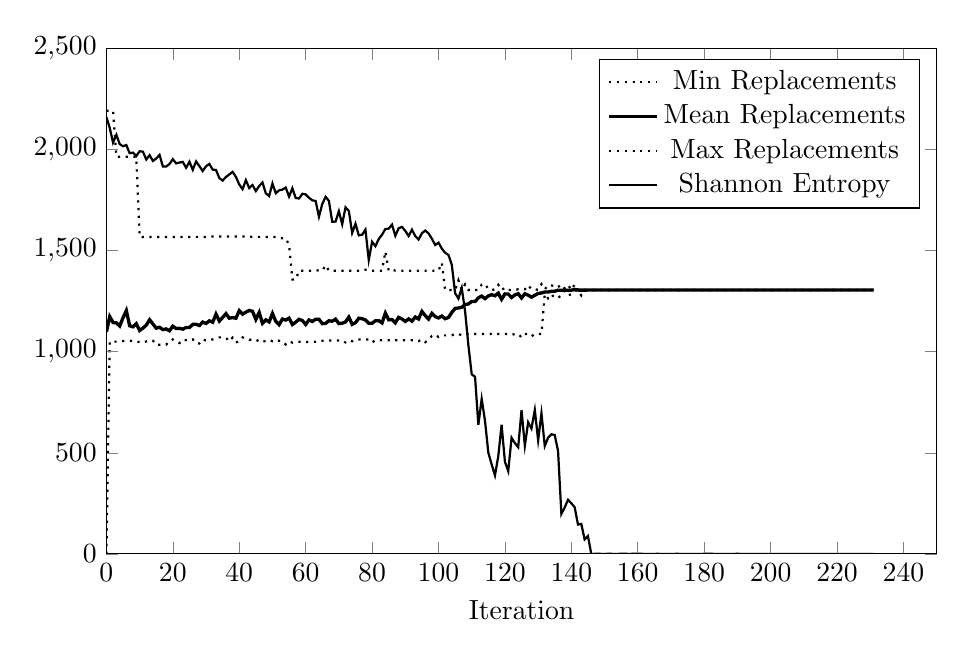
\begin{tikzpicture}[trim left=-1cm]

\definecolor{color1}{rgb}{0.75,0,0.75}
\definecolor{color0}{rgb}{0,0.75,0.75}

\begin{axis}[
width=\textwidth,
height=8cm,
xlabel={Iteration},
xmin=0, xmax=250,
ymin=0, ymax=2500,
axis on top,
legend entries={{Min Replacements},{Mean Replacements},{Max Replacements},{Shannon Entropy}}
]
\addplot [dotted, thick]
coordinates {
(0,0)
(1,1050)
(2,1050)
(3,1050)
(4,1050)
(5,1053)
(6,1055)
(7,1055)
(8,1053)
(9,1048)
(10,1049)
(11,1045)
(12,1051)
(13,1055)
(14,1055)
(15,1034)
(16,1035)
(17,1035)
(18,1035)
(19,1054)
(20,1061)
(21,1050)
(22,1043)
(23,1060)
(24,1057)
(25,1054)
(26,1061)
(27,1042)
(28,1041)
(29,1061)
(30,1055)
(31,1060)
(32,1061)
(33,1067)
(34,1071)
(35,1071)
(36,1069)
(37,1051)
(38,1070)
(39,1046)
(40,1052)
(41,1071)
(42,1065)
(43,1059)
(44,1059)
(45,1052)
(46,1059)
(47,1049)
(48,1054)
(49,1059)
(50,1052)
(51,1059)
(52,1054)
(53,1052)
(54,1036)
(55,1051)
(56,1045)
(57,1049)
(58,1049)
(59,1049)
(60,1048)
(61,1049)
(62,1049)
(63,1049)
(64,1049)
(65,1054)
(66,1054)
(67,1056)
(68,1056)
(69,1055)
(70,1056)
(71,1056)
(72,1046)
(73,1057)
(74,1052)
(75,1060)
(76,1060)
(77,1060)
(78,1060)
(79,1060)
(80,1046)
(81,1057)
(82,1057)
(83,1057)
(84,1057)
(85,1057)
(86,1052)
(87,1057)
(88,1057)
(89,1057)
(90,1057)
(91,1057)
(92,1057)
(93,1057)
(94,1053)
(95,1060)
(96,1047)
(97,1059)
(98,1078)
(99,1085)
(100,1073)
(101,1081)
(102,1081)
(103,1081)
(104,1081)
(105,1088)
(106,1088)
(107,1081)
(108,1088)
(109,1088)
(110,1088)
(111,1088)
(112,1088)
(113,1088)
(114,1088)
(115,1088)
(116,1088)
(117,1084)
(118,1088)
(119,1088)
(120,1088)
(121,1088)
(122,1083)
(123,1088)
(124,1088)
(125,1071)
(126,1088)
(127,1088)
(128,1076)
(129,1088)
(130,1088)
(131,1088)
(132,1285)
(133,1264)
(134,1284)
(135,1266)
(136,1266)
(137,1280)
(138,1302)
(139,1281)
(140,1283)
(141,1303)
(142,1303)
(143,1278)
(144,1302)
(145,1304)
(146,1304)
(147,1304)
(148,1304)
(149,1305)
(150,1305)
(151,1304)
(152,1304)
(153,1305)
(154,1305)
(155,1304)
(156,1305)
(157,1304)
(158,1305)
(159,1304)
(160,1304)
(161,1305)
(162,1305)
(163,1304)
(164,1304)
(165,1305)
(166,1304)
(167,1305)
(168,1305)
(169,1305)
(170,1305)
(171,1305)
(172,1304)
(173,1305)
(174,1305)
(175,1305)
(176,1305)
(177,1305)
(178,1305)
(179,1305)
(180,1304)
(181,1305)
(182,1304)
(183,1304)
(184,1305)
(185,1305)
(186,1305)
(187,1304)
(188,1305)
(189,1305)
(190,1304)
(191,1305)
(192,1305)
(193,1305)
(194,1305)
(195,1305)
(196,1305)
(197,1305)
(198,1305)
(199,1305)
(200,1305)
(201,1304)
(202,1305)
(203,1305)
(204,1304)
(205,1305)
(206,1305)
(207,1305)
(208,1305)
(209,1305)
(210,1305)
(211,1305)
(212,1304)
(213,1305)
(214,1305)
(215,1305)
(216,1305)
(217,1305)
(218,1305)
(219,1305)
(220,1305)
(221,1305)
(222,1305)
(223,1305)
(224,1305)
(225,1305)
(226,1305)
(227,1305)
(228,1305)
(229,1305)
(230,1305)
(231,1305)

};
\addplot [very thick]
coordinates {
(0,1098.22)
(1,1173.68)
(2,1144.42)
(3,1142.98)
(4,1127.16)
(5,1168.1)
(6,1203.62)
(7,1128.46)
(8,1123.28)
(9,1139.1)
(10,1104.96)
(11,1116.96)
(12,1131.36)
(13,1158.22)
(14,1137.6)
(15,1116.5)
(16,1120.98)
(17,1109.32)
(18,1112.78)
(19,1103.8)
(20,1126.4)
(21,1114.94)
(22,1115.8)
(23,1111.76)
(24,1120.2)
(25,1119.42)
(26,1135.34)
(27,1135.68)
(28,1129.74)
(29,1146.6)
(30,1139.78)
(31,1152.72)
(32,1146.18)
(33,1186.16)
(34,1151.74)
(35,1169.36)
(36,1188.42)
(37,1166.14)
(38,1168.88)
(39,1165.7)
(40,1203.2)
(41,1185.78)
(42,1195.92)
(43,1204.5)
(44,1199.74)
(45,1159.98)
(46,1194.22)
(47,1140.64)
(48,1157.76)
(49,1147.12)
(50,1189.06)
(51,1150.18)
(52,1134.06)
(53,1161.74)
(54,1156.58)
(55,1166.18)
(56,1134.64)
(57,1146.38)
(58,1160.34)
(59,1154.3)
(60,1135.06)
(61,1157.2)
(62,1149.86)
(63,1160.64)
(64,1160.92)
(65,1138.9)
(66,1140.44)
(67,1153.08)
(68,1150.88)
(69,1161.12)
(70,1139.32)
(71,1141.14)
(72,1147.56)
(73,1171.5)
(74,1135.4)
(75,1143.44)
(76,1166.02)
(77,1163.2)
(78,1157.32)
(79,1140.5)
(80,1140.78)
(81,1153.5)
(82,1153.6)
(83,1142.5)
(84,1191)
(85,1157.78)
(86,1159.36)
(87,1143.22)
(88,1169.92)
(89,1162.12)
(90,1149.84)
(91,1162.38)
(92,1151.36)
(93,1171.74)
(94,1161.9)
(95,1199.36)
(96,1178.86)
(97,1161.56)
(98,1189.62)
(99,1174)
(100,1167.16)
(101,1176.46)
(102,1163.36)
(103,1169.42)
(104,1194.26)
(105,1214.36)
(106,1216.3)
(107,1219.8)
(108,1233.62)
(109,1236.1)
(110,1248.82)
(111,1248.26)
(112,1266.64)
(113,1275.34)
(114,1262.7)
(115,1276.06)
(116,1282.22)
(117,1276.74)
(118,1289.94)
(119,1259.32)
(120,1285.96)
(121,1285.08)
(122,1268.36)
(123,1281.06)
(124,1287.1)
(125,1265.86)
(126,1286.86)
(127,1279.66)
(128,1269.86)
(129,1279.4)
(130,1288.08)
(131,1290.58)
(132,1295.62)
(133,1295.4)
(134,1298.76)
(135,1299.54)
(136,1304.5)
(137,1304.02)
(138,1305.02)
(139,1303.68)
(140,1304.32)
(141,1308.34)
(142,1305.02)
(143,1304.58)
(144,1304.76)
(145,1305)
(146,1304.98)
(147,1304.98)
(148,1305)
(149,1305)
(150,1305)
(151,1305)
(152,1304.96)
(153,1305)
(154,1305)
(155,1305)
(156,1305.04)
(157,1304.98)
(158,1305.02)
(159,1304.96)
(160,1305)
(161,1305.04)
(162,1305)
(163,1304.98)
(164,1304.98)
(165,1305)
(166,1305)
(167,1305)
(168,1305)
(169,1305)
(170,1305.02)
(171,1305.02)
(172,1304.96)
(173,1305)
(174,1305)
(175,1305)
(176,1305)
(177,1305)
(178,1305)
(179,1305)
(180,1304.96)
(181,1305.04)
(182,1304.96)
(183,1304.98)
(184,1305)
(185,1305)
(186,1305)
(187,1304.98)
(188,1305)
(189,1305)
(190,1304.98)
(191,1305)
(192,1305.02)
(193,1305)
(194,1305)
(195,1305)
(196,1305)
(197,1305)
(198,1305)
(199,1305)
(200,1305)
(201,1304.98)
(202,1305)
(203,1305)
(204,1304.98)
(205,1305)
(206,1305)
(207,1305)
(208,1305)
(209,1305)
(210,1305)
(211,1305)
(212,1304.98)
(213,1305)
(214,1305)
(215,1305)
(216,1305)
(217,1305)
(218,1305)
(219,1305)
(220,1305)
(221,1305)
(222,1305)
(223,1305)
(224,1305)
(225,1305)
(226,1305)
(227,1305)
(228,1305)
(229,1305)
(230,1305)
(231,1305)

};
\addplot [dotted, thick]
coordinates {
(0,2192)
(1,2192)
(2,2192)
(3,1965)
(4,1965)
(5,1965)
(6,1965)
(7,1965)
(8,1965)
(9,1965)
(10,1568)
(11,1568)
(12,1568)
(13,1568)
(14,1568)
(15,1568)
(16,1568)
(17,1568)
(18,1568)
(19,1568)
(20,1568)
(21,1568)
(22,1568)
(23,1568)
(24,1568)
(25,1568)
(26,1568)
(27,1568)
(28,1568)
(29,1568)
(30,1568)
(31,1570)
(32,1570)
(33,1570)
(34,1570)
(35,1570)
(36,1570)
(37,1570)
(38,1570)
(39,1570)
(40,1570)
(41,1570)
(42,1570)
(43,1570)
(44,1568)
(45,1568)
(46,1568)
(47,1568)
(48,1568)
(49,1568)
(50,1568)
(51,1568)
(52,1561)
(53,1561)
(54,1561)
(55,1529)
(56,1357)
(57,1357)
(58,1401)
(59,1401)
(60,1401)
(61,1401)
(62,1401)
(63,1404)
(64,1401)
(65,1401)
(66,1428)
(67,1401)
(68,1401)
(69,1401)
(70,1401)
(71,1401)
(72,1401)
(73,1401)
(74,1401)
(75,1401)
(76,1401)
(77,1401)
(78,1406)
(79,1401)
(80,1401)
(81,1401)
(82,1401)
(83,1401)
(84,1496)
(85,1401)
(86,1407)
(87,1401)
(88,1401)
(89,1401)
(90,1401)
(91,1401)
(92,1401)
(93,1401)
(94,1401)
(95,1401)
(96,1401)
(97,1401)
(98,1401)
(99,1401)
(100,1401)
(101,1440)
(102,1305)
(103,1305)
(104,1305)
(105,1305)
(106,1353)
(107,1305)
(108,1333)
(109,1305)
(110,1310)
(111,1305)
(112,1305)
(113,1332)
(114,1336)
(115,1310)
(116,1305)
(117,1309)
(118,1331)
(119,1305)
(120,1317)
(121,1305)
(122,1305)
(123,1305)
(124,1309)
(125,1309)
(126,1309)
(127,1329)
(128,1309)
(129,1309)
(130,1306)
(131,1334)
(132,1309)
(133,1329)
(134,1328)
(135,1325)
(136,1330)
(137,1306)
(138,1315)
(139,1331)
(140,1306)
(141,1333)
(142,1307)
(143,1308)
(144,1306)
(145,1306)
(146,1305)
(147,1305)
(148,1306)
(149,1305)
(150,1305)
(151,1306)
(152,1305)
(153,1305)
(154,1305)
(155,1306)
(156,1306)
(157,1305)
(158,1306)
(159,1306)
(160,1306)
(161,1306)
(162,1305)
(163,1305)
(164,1305)
(165,1305)
(166,1306)
(167,1305)
(168,1305)
(169,1305)
(170,1306)
(171,1306)
(172,1305)
(173,1305)
(174,1305)
(175,1305)
(176,1305)
(177,1305)
(178,1305)
(179,1305)
(180,1305)
(181,1306)
(182,1305)
(183,1305)
(184,1305)
(185,1305)
(186,1305)
(187,1305)
(188,1305)
(189,1305)
(190,1306)
(191,1305)
(192,1306)
(193,1305)
(194,1305)
(195,1305)
(196,1305)
(197,1305)
(198,1305)
(199,1305)
(200,1305)
(201,1305)
(202,1305)
(203,1305)
(204,1305)
(205,1305)
(206,1305)
(207,1305)
(208,1305)
(209,1305)
(210,1305)
(211,1305)
(212,1305)
(213,1305)
(214,1305)
(215,1305)
(216,1305)
(217,1305)
(218,1305)
(219,1305)
(220,1305)
(221,1305)
(222,1305)
(223,1305)
(224,1305)
(225,1305)
(226,1305)
(227,1305)
(228,1305)
(229,1305)
(230,1305)
(231,1305)

};
\addplot [thick]
coordinates {
(0,2160.68184796898)
(1,2107.01650496597)
(2,2034.67711368443)
(3,2073.13233216073)
(4,2027.09750756848)
(5,2016.66915001637)
(6,2022.17352598052)
(7,1982.04988579901)
(8,1985.01008454357)
(9,1968.14006807668)
(10,1991.73898151782)
(11,1989.55244040009)
(12,1950.84894505685)
(13,1972.26478538619)
(14,1943.76317640536)
(15,1955.79209701649)
(16,1973.69561355895)
(17,1916.56460722881)
(18,1916.09535595699)
(19,1928.75483322777)
(20,1952.45980025382)
(21,1931.69422841475)
(22,1935.68446401047)
(23,1939.04953649837)
(24,1909.95390015891)
(25,1939.94078698853)
(26,1900.21410245463)
(27,1941.42549520962)
(28,1918.06816210788)
(29,1893.85210423011)
(30,1917.53386527792)
(31,1929.09323196891)
(32,1900.80135909605)
(33,1898.97355664936)
(34,1859.4318574017)
(35,1846.73511426727)
(36,1864.30864951943)
(37,1876.93158042825)
(38,1889.73393616656)
(39,1864.82023759697)
(40,1827.54035104113)
(41,1804.47305248458)
(42,1848.68019885512)
(43,1809.81033180087)
(44,1824.65866544311)
(45,1794.97425263299)
(46,1819.53987233204)
(47,1837.28881388303)
(48,1783.59625710631)
(49,1769.92723926931)
(50,1832.17111232674)
(51,1784.06963383456)
(52,1798.18681335118)
(53,1802.12876860156)
(54,1812.19709955257)
(55,1767.63694916515)
(56,1808.36388766153)
(57,1760.45432560978)
(58,1757.87593976002)
(59,1781.25977280095)
(60,1778.3857900454)
(61,1761.63239542485)
(62,1749.16180968578)
(63,1745.7308874784)
(64,1667.93922289779)
(65,1730.91384898639)
(66,1766.28442502785)
(67,1746.04745947448)
(68,1642.93560862484)
(69,1643.8274662032)
(70,1695.16532406806)
(71,1631.00214697987)
(72,1714.45245577551)
(73,1695.89821693383)
(74,1587.77855302626)
(75,1633.07896160204)
(76,1575.4640207064)
(77,1578.90492418148)
(78,1603.74512252056)
(79,1453.79182293838)
(80,1544.00070756925)
(81,1522.29374406686)
(82,1557.4872731119)
(83,1579.26721938683)
(84,1607.17997487786)
(85,1609.03998581013)
(86,1628.67029629546)
(87,1573.54211076139)
(88,1610.7695201208)
(89,1617.65092988149)
(90,1597.69068424914)
(91,1572.37448251783)
(92,1603.52357238857)
(93,1571.91001153489)
(94,1555.09632784989)
(95,1586.05453230179)
(96,1599.48158294417)
(97,1585.45698130318)
(98,1559.2846112441)
(99,1528.12168862713)
(100,1539.60578049928)
(101,1510.14276355309)
(102,1489.28557227771)
(103,1478.71624620477)
(104,1430.86332144163)
(105,1289.91514411884)
(106,1262.89250229568)
(107,1315.96178106345)
(108,1200.4560124766)
(109,1032.40261192552)
(110,888.172309566672)
(111,876.431320344367)
(112,638.322232499761)
(113,767.102526381945)
(114,658.070665852564)
(115,501.132632366283)
(116,443.125444275208)
(117,388.337476083347)
(118,483.314942691348)
(119,639.470540446886)
(120,456.036704326745)
(121,409.310639810898)
(122,574.614097250359)
(123,547.890577437779)
(124,527.545245426385)
(125,710.419568594422)
(126,534.923767842432)
(127,650.902618453724)
(128,620.22381372521)
(129,711.924303666527)
(130,561.673933947029)
(131,695.457373822375)
(132,533.905842132745)
(133,574.735287571342)
(134,591.696553970246)
(135,587.84724639526)
(136,508.803909944198)
(137,197.560862622551)
(138,229.65566080458)
(139,267.669898606426)
(140,250.226735954697)
(141,231.03022229714)
(142,145.186317631279)
(143,148.032947456323)
(144,71.7857486605586)
(145,88.5683585233182)
(146,0.141440542541818)
(147,0.141440542541818)
(148,0.767465463248466)
(149,0)
(150,0)
(151,0.282881085083638)
(152,0.242292189082412)
(153,0)
(154,0)
(155,0.52517327416605)
(156,0.282881085083641)
(157,0.141440542541818)
(158,0.141440542541821)
(159,0.525173274166051)
(160,0.282881085083638)
(161,0.282881085083641)
(162,0)
(163,0.141440542541818)
(164,0.141440542541818)
(165,0)
(166,0.282881085083638)
(167,0)
(168,0)
(169,0)
(170,0.141440542541821)
(171,0.141440542541821)
(172,0.242292189082412)
(173,0)
(174,0)
(175,0)
(176,0)
(177,0)
(178,0)
(179,0)
(180,0.242292189082412)
(181,0.242292189082415)
(182,0.242292189082412)
(183,0.141440542541818)
(184,0)
(185,0)
(186,0)
(187,0.141440542541818)
(188,0)
(189,0)
(190,0.383732731624233)
(191,0)
(192,0.141440542541821)
(193,0)
(194,0)
(195,0)
(196,0)
(197,0)
(198,0)
(199,0)
(200,0)
(201,0.141440542541818)
(202,0)
(203,0)
(204,0.141440542541818)
(205,0)
(206,0)
(207,0)
(208,0)
(209,0)
(210,0)
(211,0)
(212,0.141440542541818)
(213,0)
(214,0)
(215,0)
(216,0)
(217,0)
(218,0)
(219,0)
(220,0)
(221,0)
(222,0)
(223,0)
(224,0)
(225,0)
(226,0)
(227,0)
(228,0)
(229,0)
(230,0)
(231,0)

};
\path [draw=black, fill opacity=0] (axis cs:13,2500)--(axis cs:13,2500);

\path [draw=black, fill opacity=0] (axis cs:250,13)--(axis cs:250,13);

\path [draw=black, fill opacity=0] (axis cs:13,0)--(axis cs:13,0);

\path [draw=black, fill opacity=0] (axis cs:0,13)--(axis cs:0,13);

\end{axis}

\end{tikzpicture}


  \vspace{1cm}

  % This file was created by matplotlib v0.1.0.
% Copyright (c) 2010--2014, Nico Schlömer <nico.schloemer@gmail.com>
% All rights reserved.
%
% The lastest updates can be retrieved from
%
% https://github.com/nschloe/matplotlib2tikz
%
% where you can also submit bug reports and leavecomments.
%
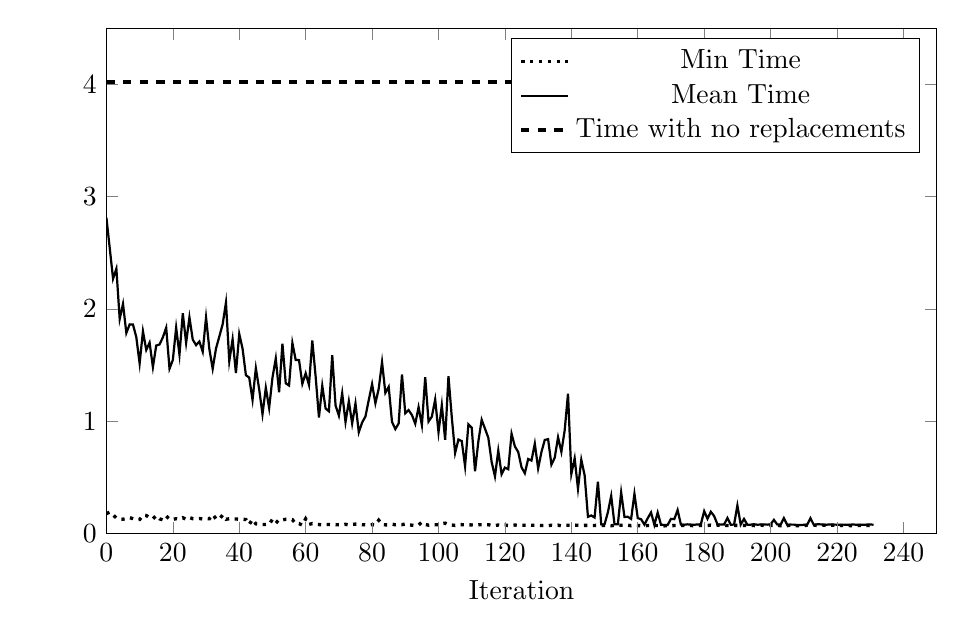
\begin{tikzpicture}[trim left=-1cm]

\begin{axis}[
width=\textwidth,
height=8cm,
xlabel={Iteration},
xmin=0, xmax=250,
ymin=0, ymax=4.5,
axis on top,
legend entries={{Min Time},{Mean Time},{Time with no replacements}}
]
\addplot [dotted, very thick]
coordinates {
(0,0.177843)
(1,0.191291)
(2,0.16781)
(3,0.138891)
(4,0.127859)
(5,0.128776)
(6,0.133265)
(7,0.142724)
(8,0.133172)
(9,0.123475)
(10,0.125565)
(11,0.163929)
(12,0.161608)
(13,0.140589)
(14,0.131784)
(15,0.160637)
(16,0.131361)
(17,0.121875)
(18,0.156417)
(19,0.128463)
(20,0.126833)
(21,0.133051)
(22,0.128424)
(23,0.141356)
(24,0.12724)
(25,0.143519)
(26,0.13281)
(27,0.130949)
(28,0.134505)
(29,0.130423)
(30,0.13432)
(31,0.132152)
(32,0.169632)
(33,0.131783)
(34,0.127189)
(35,0.165769)
(36,0.127767)
(37,0.132244)
(38,0.130598)
(39,0.13069)
(40,0.127078)
(41,0.128342)
(42,0.12551)
(43,0.082532)
(44,0.126714)
(45,0.087025)
(46,0.082384)
(47,0.081754)
(48,0.080801)
(49,0.08244)
(50,0.126208)
(51,0.092565)
(52,0.125642)
(53,0.121235)
(54,0.127919)
(55,0.127001)
(56,0.124199)
(57,0.087746)
(58,0.089106)
(59,0.075415)
(60,0.131512)
(61,0.081658)
(62,0.08982)
(63,0.082581)
(64,0.080649)
(65,0.078136)
(66,0.080833)
(67,0.081117)
(68,0.080938)
(69,0.079933)
(70,0.078006)
(71,0.078399)
(72,0.082834)
(73,0.077308)
(74,0.082215)
(75,0.084864)
(76,0.08374)
(77,0.079021)
(78,0.077942)
(79,0.077833)
(80,0.07919)
(81,0.076969)
(82,0.119053)
(83,0.080996)
(84,0.077999)
(85,0.078014)
(86,0.084449)
(87,0.078628)
(88,0.08187)
(89,0.080055)
(90,0.085827)
(91,0.077894)
(92,0.074914)
(93,0.070864)
(94,0.076605)
(95,0.101984)
(96,0.081369)
(97,0.075131)
(98,0.079316)
(99,0.078199)
(100,0.079845)
(101,0.08873)
(102,0.092883)
(103,0.079631)
(104,0.076531)
(105,0.072896)
(106,0.080277)
(107,0.079712)
(108,0.079104)
(109,0.078497)
(110,0.077267)
(111,0.076798)
(112,0.078396)
(113,0.079082)
(114,0.079566)
(115,0.079635)
(116,0.072892)
(117,0.072255)
(118,0.076718)
(119,0.072269)
(120,0.075931)
(121,0.072789)
(122,0.072508)
(123,0.076751)
(124,0.07268)
(125,0.074929)
(126,0.075223)
(127,0.077626)
(128,0.07445)
(129,0.07473)
(130,0.073717)
(131,0.072527)
(132,0.07253)
(133,0.070948)
(134,0.074623)
(135,0.071114)
(136,0.075441)
(137,0.06838)
(138,0.074242)
(139,0.074767)
(140,0.072318)
(141,0.075526)
(142,0.074127)
(143,0.072152)
(144,0.073624)
(145,0.073495)
(146,0.072631)
(147,0.072684)
(148,0.0746)
(149,0.073605)
(150,0.071515)
(151,0.073553)
(152,0.070123)
(153,0.073898)
(154,0.073564)
(155,0.074554)
(156,0.074699)
(157,0.075098)
(158,0.070274)
(159,0.073819)
(160,0.071435)
(161,0.071293)
(162,0.069582)
(163,0.072579)
(164,0.071627)
(165,0.07145)
(166,0.07169)
(167,0.071333)
(168,0.069006)
(169,0.071749)
(170,0.070236)
(171,0.07177)
(172,0.073247)
(173,0.073225)
(174,0.073207)
(175,0.073625)
(176,0.072359)
(177,0.069215)
(178,0.072349)
(179,0.072643)
(180,0.07425)
(181,0.072674)
(182,0.075305)
(183,0.069772)
(184,0.075079)
(185,0.0736)
(186,0.073262)
(187,0.071952)
(188,0.070201)
(189,0.073502)
(190,0.073332)
(191,0.074606)
(192,0.072768)
(193,0.071152)
(194,0.073645)
(195,0.072398)
(196,0.06736)
(197,0.074862)
(198,0.072795)
(199,0.073624)
(200,0.072974)
(201,0.072914)
(202,0.07427)
(203,0.07002)
(204,0.073678)
(205,0.070594)
(206,0.075039)
(207,0.0726)
(208,0.069893)
(209,0.07086)
(210,0.070504)
(211,0.074518)
(212,0.071306)
(213,0.074234)
(214,0.073356)
(215,0.073577)
(216,0.074927)
(217,0.074322)
(218,0.073997)
(219,0.074682)
(220,0.072866)
(221,0.072727)
(222,0.072617)
(223,0.074963)
(224,0.070865)
(225,0.068987)
(226,0.071643)
(227,0.073107)
(228,0.070417)
(229,0.071589)
(230,0.072118)
(231,0.072681)

};
\addplot [thick]
coordinates {
(0,2.8132832)
(1,2.5423655)
(2,2.26977936)
(3,2.35830814)
(4,1.91069088)
(5,2.0455562)
(6,1.78611638)
(7,1.8630946)
(8,1.86137304)
(9,1.74979092)
(10,1.51436294)
(11,1.80148814)
(12,1.63523896)
(13,1.70059456)
(14,1.4821947)
(15,1.67466596)
(16,1.68425732)
(17,1.74776198)
(18,1.8336578)
(19,1.46874044)
(20,1.54604916)
(21,1.8339739)
(22,1.59350644)
(23,1.96199178)
(24,1.69830898)
(25,1.92577802)
(26,1.72737414)
(27,1.67830098)
(28,1.71049284)
(29,1.61977916)
(30,1.9249023)
(31,1.64242926)
(32,1.46824514)
(33,1.64796326)
(34,1.75515184)
(35,1.86374552)
(36,2.05746966)
(37,1.5352368)
(38,1.73048114)
(39,1.42983724)
(40,1.77830386)
(41,1.64681568)
(42,1.41066582)
(43,1.38941752)
(44,1.1907695)
(45,1.47250662)
(46,1.28544024)
(47,1.06388328)
(48,1.29872148)
(49,1.11849912)
(50,1.38818282)
(51,1.55962288)
(52,1.25852796)
(53,1.69164948)
(54,1.33879666)
(55,1.31892424)
(56,1.69708744)
(57,1.54615286)
(58,1.54480756)
(59,1.33412772)
(60,1.42721734)
(61,1.32371818)
(62,1.71898308)
(63,1.39929954)
(64,1.03421094)
(65,1.31645428)
(66,1.11368256)
(67,1.0894998)
(68,1.58943274)
(69,1.14078124)
(70,1.05044974)
(71,1.25012426)
(72,0.99305678)
(73,1.17863604)
(74,0.9802021)
(75,1.15854706)
(76,0.902561)
(77,0.98958218)
(78,1.04295192)
(79,1.18969436)
(80,1.33134746)
(81,1.16104712)
(82,1.29014174)
(83,1.5274728)
(84,1.252995)
(85,1.30666308)
(86,0.99473888)
(87,0.93080514)
(88,0.98061154)
(89,1.4159979)
(90,1.07149788)
(91,1.0995593)
(92,1.05581408)
(93,0.97812726)
(94,1.12620282)
(95,0.9653786)
(96,1.39366824)
(97,0.99813918)
(98,1.0417172)
(99,1.19464146)
(100,0.90222006)
(101,1.14457732)
(102,0.83516074)
(103,1.40247672)
(104,1.03605252)
(105,0.71783708)
(106,0.83744174)
(107,0.82360296)
(108,0.5998113)
(109,0.97289088)
(110,0.94332702)
(111,0.55587512)
(112,0.82089848)
(113,1.01349258)
(114,0.93440722)
(115,0.85324804)
(116,0.63824588)
(117,0.50930496)
(118,0.73958936)
(119,0.52887582)
(120,0.5877064)
(121,0.57339262)
(122,0.88940818)
(123,0.77594368)
(124,0.72704956)
(125,0.59038648)
(126,0.53763544)
(127,0.6646116)
(128,0.65074724)
(129,0.80116758)
(130,0.58012328)
(131,0.72663908)
(132,0.83414504)
(133,0.84110498)
(134,0.61401418)
(135,0.67603092)
(136,0.85791644)
(137,0.72810556)
(138,0.92049996)
(139,1.24589088)
(140,0.5306256)
(141,0.67001946)
(142,0.39955588)
(143,0.65797922)
(144,0.51925896)
(145,0.14955662)
(146,0.16154308)
(147,0.14341334)
(148,0.4619641)
(149,0.08212676)
(150,0.0822266)
(151,0.18944366)
(152,0.33539878)
(153,0.08276878)
(154,0.08228256)
(155,0.36694364)
(156,0.14859362)
(157,0.14945204)
(158,0.13096234)
(159,0.35422754)
(160,0.13792366)
(161,0.12792786)
(162,0.0800056)
(163,0.13692352)
(164,0.18861064)
(165,0.07792614)
(166,0.18706618)
(167,0.07848558)
(168,0.07766278)
(169,0.07674388)
(170,0.1313438)
(171,0.12886728)
(172,0.20978318)
(173,0.07992994)
(174,0.07882128)
(175,0.08259488)
(176,0.08005828)
(177,0.07857476)
(178,0.08147152)
(179,0.08291728)
(180,0.20004374)
(181,0.13238672)
(182,0.1941681)
(183,0.15666032)
(184,0.08294564)
(185,0.08008204)
(186,0.08116324)
(187,0.13949818)
(188,0.07933622)
(189,0.08023862)
(190,0.25040668)
(191,0.08034712)
(192,0.1307059)
(193,0.07859296)
(194,0.07964926)
(195,0.08349462)
(196,0.07929936)
(197,0.08064212)
(198,0.08141762)
(199,0.0798378)
(200,0.0822315)
(201,0.12245506)
(202,0.0815155)
(203,0.07964828)
(204,0.13825994)
(205,0.07911928)
(206,0.0802846)
(207,0.07990072)
(208,0.07673912)
(209,0.07642278)
(210,0.0783635)
(211,0.07877114)
(212,0.1372843)
(213,0.0785827)
(214,0.08242106)
(215,0.0823984)
(216,0.07989238)
(217,0.07966062)
(218,0.08196598)
(219,0.08023464)
(220,0.07973294)
(221,0.07821416)
(222,0.0799758)
(223,0.0791715)
(224,0.07995094)
(225,0.08077778)
(226,0.07878352)
(227,0.07973808)
(228,0.07854718)
(229,0.08025846)
(230,0.08115192)
(231,0.07917116)

};
\addplot [dashed, very thick]
coordinates {
(0,4.0212)
(1,4.0212)
(2,4.0212)
(3,4.0212)
(4,4.0212)
(5,4.0212)
(6,4.0212)
(7,4.0212)
(8,4.0212)
(9,4.0212)
(10,4.0212)
(11,4.0212)
(12,4.0212)
(13,4.0212)
(14,4.0212)
(15,4.0212)
(16,4.0212)
(17,4.0212)
(18,4.0212)
(19,4.0212)
(20,4.0212)
(21,4.0212)
(22,4.0212)
(23,4.0212)
(24,4.0212)
(25,4.0212)
(26,4.0212)
(27,4.0212)
(28,4.0212)
(29,4.0212)
(30,4.0212)
(31,4.0212)
(32,4.0212)
(33,4.0212)
(34,4.0212)
(35,4.0212)
(36,4.0212)
(37,4.0212)
(38,4.0212)
(39,4.0212)
(40,4.0212)
(41,4.0212)
(42,4.0212)
(43,4.0212)
(44,4.0212)
(45,4.0212)
(46,4.0212)
(47,4.0212)
(48,4.0212)
(49,4.0212)
(50,4.0212)
(51,4.0212)
(52,4.0212)
(53,4.0212)
(54,4.0212)
(55,4.0212)
(56,4.0212)
(57,4.0212)
(58,4.0212)
(59,4.0212)
(60,4.0212)
(61,4.0212)
(62,4.0212)
(63,4.0212)
(64,4.0212)
(65,4.0212)
(66,4.0212)
(67,4.0212)
(68,4.0212)
(69,4.0212)
(70,4.0212)
(71,4.0212)
(72,4.0212)
(73,4.0212)
(74,4.0212)
(75,4.0212)
(76,4.0212)
(77,4.0212)
(78,4.0212)
(79,4.0212)
(80,4.0212)
(81,4.0212)
(82,4.0212)
(83,4.0212)
(84,4.0212)
(85,4.0212)
(86,4.0212)
(87,4.0212)
(88,4.0212)
(89,4.0212)
(90,4.0212)
(91,4.0212)
(92,4.0212)
(93,4.0212)
(94,4.0212)
(95,4.0212)
(96,4.0212)
(97,4.0212)
(98,4.0212)
(99,4.0212)
(100,4.0212)
(101,4.0212)
(102,4.0212)
(103,4.0212)
(104,4.0212)
(105,4.0212)
(106,4.0212)
(107,4.0212)
(108,4.0212)
(109,4.0212)
(110,4.0212)
(111,4.0212)
(112,4.0212)
(113,4.0212)
(114,4.0212)
(115,4.0212)
(116,4.0212)
(117,4.0212)
(118,4.0212)
(119,4.0212)
(120,4.0212)
(121,4.0212)
(122,4.0212)
(123,4.0212)
(124,4.0212)
(125,4.0212)
(126,4.0212)
(127,4.0212)
(128,4.0212)
(129,4.0212)
(130,4.0212)
(131,4.0212)
(132,4.0212)
(133,4.0212)
(134,4.0212)
(135,4.0212)
(136,4.0212)
(137,4.0212)
(138,4.0212)
(139,4.0212)
(140,4.0212)
(141,4.0212)
(142,4.0212)
(143,4.0212)
(144,4.0212)
(145,4.0212)
(146,4.0212)
(147,4.0212)
(148,4.0212)
(149,4.0212)
(150,4.0212)
(151,4.0212)
(152,4.0212)
(153,4.0212)
(154,4.0212)
(155,4.0212)
(156,4.0212)
(157,4.0212)
(158,4.0212)
(159,4.0212)
(160,4.0212)
(161,4.0212)
(162,4.0212)
(163,4.0212)
(164,4.0212)
(165,4.0212)
(166,4.0212)
(167,4.0212)
(168,4.0212)
(169,4.0212)
(170,4.0212)
(171,4.0212)
(172,4.0212)
(173,4.0212)
(174,4.0212)
(175,4.0212)
(176,4.0212)
(177,4.0212)
(178,4.0212)
(179,4.0212)
(180,4.0212)
(181,4.0212)
(182,4.0212)
(183,4.0212)
(184,4.0212)
(185,4.0212)
(186,4.0212)
(187,4.0212)
(188,4.0212)
(189,4.0212)
(190,4.0212)
(191,4.0212)
(192,4.0212)
(193,4.0212)
(194,4.0212)
(195,4.0212)
(196,4.0212)
(197,4.0212)
(198,4.0212)
(199,4.0212)
(200,4.0212)
(201,4.0212)
(202,4.0212)
(203,4.0212)
(204,4.0212)
(205,4.0212)
(206,4.0212)
(207,4.0212)
(208,4.0212)
(209,4.0212)
(210,4.0212)
(211,4.0212)
(212,4.0212)
(213,4.0212)
(214,4.0212)
(215,4.0212)
(216,4.0212)
(217,4.0212)
(218,4.0212)
(219,4.0212)
(220,4.0212)
(221,4.0212)
(222,4.0212)
(223,4.0212)
(224,4.0212)
(225,4.0212)
(226,4.0212)
(227,4.0212)
(228,4.0212)
(229,4.0212)
(230,4.0212)
(231,4.0212)

};
\path [draw=black, fill opacity=0] (axis cs:13,4.5)--(axis cs:13,4.5);

\path [draw=black, fill opacity=0] (axis cs:250,13)--(axis cs:250,13);

\path [draw=black, fill opacity=0] (axis cs:13,0)--(axis cs:13,0);

\path [draw=black, fill opacity=0] (axis cs:0,13)--(axis cs:0,13);

\end{axis}

\end{tikzpicture}

  \caption{{\bf square\_1\_false--unreach--call} (\sat{}): Replacements made (top), and time taken by \textsc{MiniSat} (seconds) (bottom) on each iteration.}
  \label{fig:square_1_rep_dist}
\end{figure}

\begin{figure}[p]
  % This file was created by matplotlib v0.1.0.
% Copyright (c) 2010--2014, Nico Schlömer <nico.schloemer@gmail.com>
% All rights reserved.
%
% The lastest updates can be retrieved from
%
% https://github.com/nschloe/matplotlib2tikz
%
% where you can also submit bug reports and leavecomments.
%
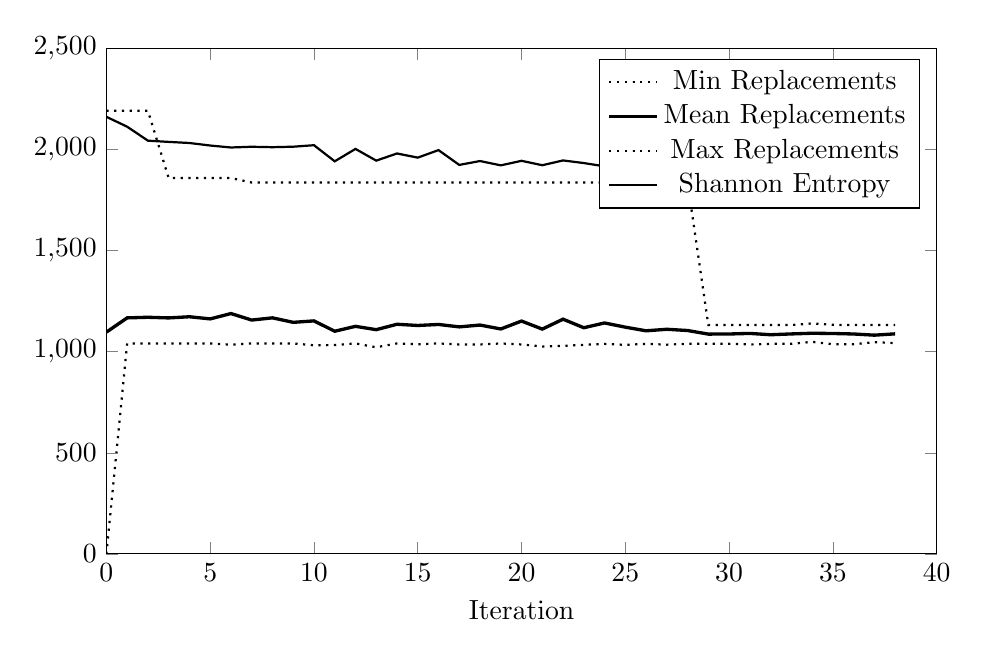
\begin{tikzpicture}[trim left=-1cm]

\definecolor{color1}{rgb}{0.75,0,0.75}
\definecolor{color0}{rgb}{0,0.75,0.75}

\begin{axis}[
width=\textwidth,
height=8cm,
xlabel={Iteration},
xmin=0, xmax=40,
ymin=0, ymax=2500,
axis on top,
legend entries={{Min Replacements},{Mean Replacements},{Max Replacements},{Shannon Entropy}}
]
\addplot [dotted, thick]
coordinates {
(0,0)
(1,1041)
(2,1041)
(3,1041)
(4,1041)
(5,1041)
(6,1035)
(7,1041)
(8,1041)
(9,1041)
(10,1032)
(11,1033)
(12,1041)
(13,1022)
(14,1041)
(15,1037)
(16,1041)
(17,1036)
(18,1036)
(19,1041)
(20,1036)
(21,1026)
(22,1029)
(23,1034)
(24,1039)
(25,1034)
(26,1039)
(27,1035)
(28,1039)
(29,1039)
(30,1039)
(31,1036)
(32,1039)
(33,1039)
(34,1049)
(35,1037)
(36,1037)
(37,1047)
(38,1043)

};
\addplot [very thick]
coordinates {
(0,1097.02)
(1,1167.5)
(2,1170.46)
(3,1167.3)
(4,1173.06)
(5,1162.42)
(6,1188.86)
(7,1156.68)
(8,1167.62)
(9,1145.42)
(10,1152.54)
(11,1101.42)
(12,1125.64)
(13,1109.14)
(14,1135.9)
(15,1129.9)
(16,1134.92)
(17,1122.94)
(18,1131.98)
(19,1112.54)
(20,1151.82)
(21,1111.92)
(22,1161.02)
(23,1118.76)
(24,1142.36)
(25,1121.54)
(26,1103.54)
(27,1111.1)
(28,1104.96)
(29,1087.2)
(30,1087.72)
(31,1090.6)
(32,1084.1)
(33,1088.1)
(34,1091.42)
(35,1090.22)
(36,1087.78)
(37,1081.96)
(38,1088.46)

};
\addplot [dotted, thick]
coordinates {
(0,2192)
(1,2192)
(2,2192)
(3,1859)
(4,1859)
(5,1859)
(6,1859)
(7,1837)
(8,1837)
(9,1837)
(10,1837)
(11,1837)
(12,1837)
(13,1837)
(14,1837)
(15,1837)
(16,1837)
(17,1837)
(18,1837)
(19,1837)
(20,1837)
(21,1837)
(22,1837)
(23,1837)
(24,1837)
(25,1837)
(26,1837)
(27,1837)
(28,1837)
(29,1132)
(30,1132)
(31,1132)
(32,1132)
(33,1132)
(34,1140)
(35,1133)
(36,1132)
(37,1132)
(38,1132)

};
\addplot [thick]
coordinates {
(0,2161.99621997945)
(1,2113.16085166022)
(2,2044.0750730143)
(3,2038.0140648874)
(4,2032.53960838096)
(5,2020.04520219301)
(6,2010.34741350398)
(7,2013.92601030156)
(8,2011.79579941526)
(9,2014.22414629607)
(10,2021.64211590226)
(11,1941.97318640824)
(12,2003.27334175338)
(13,1945.3392499272)
(14,1980.72149513039)
(15,1960.19722982837)
(16,1997.33007483401)
(17,1924.12932437937)
(18,1943.32301881714)
(19,1921.91272972286)
(20,1944.42666980454)
(21,1922.58850126645)
(22,1946.30162048225)
(23,1933.32937733597)
(24,1917.20356309781)
(25,1908.60941099222)
(26,1927.3289273151)
(27,1953.64801029677)
(28,1895.09947644068)
(29,1910.33446002315)
(30,1898.38548773066)
(31,1879.52656299292)
(32,1853.97824096427)
(33,1887.86495554381)
(34,1881.46626968771)
(35,1873.32515826854)
(36,1837.06860937504)
(37,1878.17969872628)
(38,1872.78187219633)

};
\path [draw=black, fill opacity=0] (axis cs:13,2500)--(axis cs:13,2500);

\path [draw=black, fill opacity=0] (axis cs:40,13)--(axis cs:40,13);

\path [draw=black, fill opacity=0] (axis cs:13,0)--(axis cs:13,0);

\path [draw=black, fill opacity=0] (axis cs:0,13)--(axis cs:0,13);

\end{axis}

\end{tikzpicture}


  \vspace{1cm}

  % This file was created by matplotlib v0.1.0.
% Copyright (c) 2010--2014, Nico Schlömer <nico.schloemer@gmail.com>
% All rights reserved.
%
% The lastest updates can be retrieved from
%
% https://github.com/nschloe/matplotlib2tikz
%
% where you can also submit bug reports and leavecomments.
%
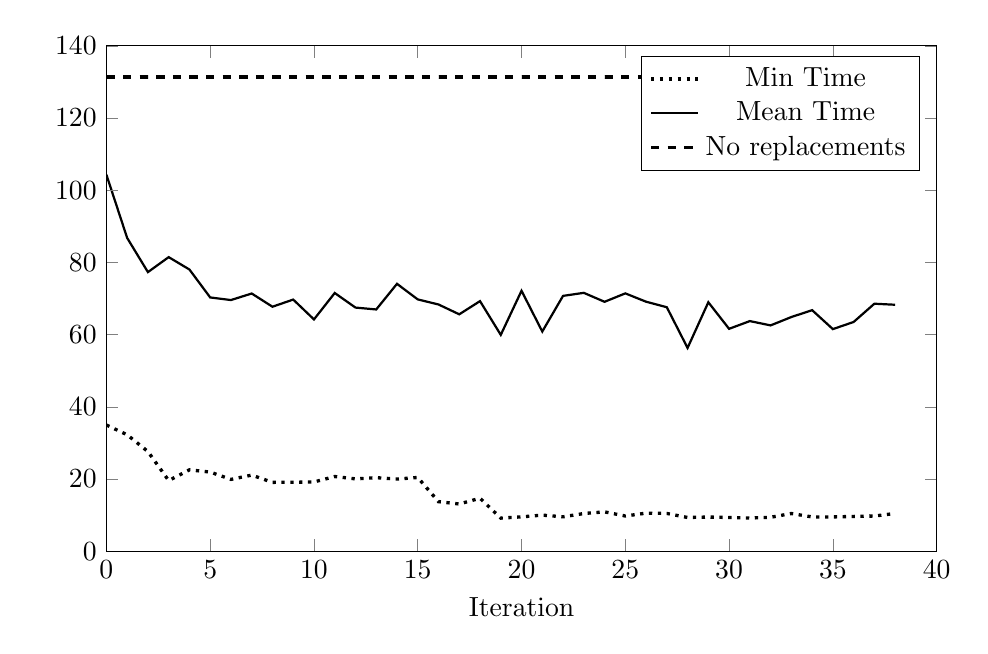
\begin{tikzpicture}[trim left=-1cm]

\begin{axis}[
width=\textwidth,
height=8cm,
xlabel={Iteration},
xmin=0, xmax=40,
ymin=0, ymax=140,
axis on top,
legend entries={{Min Time},{Mean Time},{No replacements}}
]
\addplot [dotted, very thick]
coordinates {
(0,34.9579)
(1,32.254)
(2,27.608)
(3,19.5639)
(4,22.5339)
(5,21.9218)
(6,19.8978)
(7,21.0829)
(8,19.074)
(9,19.0999)
(10,19.1823)
(11,20.69)
(12,20.0326)
(13,20.3687)
(14,19.9832)
(15,20.4251)
(16,13.7228)
(17,13.078)
(18,14.6786)
(19,9.16225)
(20,9.51277)
(21,9.99713)
(22,9.53025)
(23,10.4417)
(24,10.8963)
(25,9.75238)
(26,10.5461)
(27,10.4678)
(28,9.34168)
(29,9.46352)
(30,9.33624)
(31,9.18503)
(32,9.39811)
(33,10.4357)
(34,9.49689)
(35,9.497)
(36,9.63368)
(37,9.74072)
(38,10.4566)

};
\addplot [thick]
coordinates {
(0,104.295644)
(1,86.773332)
(2,77.310664)
(3,81.463924)
(4,78.032816)
(5,70.292842)
(6,69.572714)
(7,71.385022)
(8,67.725246)
(9,69.707306)
(10,64.206444)
(11,71.526236)
(12,67.486658)
(13,66.966018)
(14,74.072268)
(15,69.747516)
(16,68.344832)
(17,65.621184)
(18,69.279372)
(19,59.927595)
(20,72.1396894)
(21,60.8503046)
(22,70.727957)
(23,71.572178)
(24,69.088654)
(25,71.4234876)
(26,69.115268)
(27,67.582904)
(28,56.3051556)
(29,68.9650784)
(30,61.6033428)
(31,63.7455946)
(32,62.5515042)
(33,64.86731)
(34,66.7744258)
(35,61.524602)
(36,63.4963436)
(37,68.5563764)
(38,68.269344)

};
\addplot [dashed, very thick]
coordinates {
(0,131.376)
(1,131.376)
(2,131.376)
(3,131.376)
(4,131.376)
(5,131.376)
(6,131.376)
(7,131.376)
(8,131.376)
(9,131.376)
(10,131.376)
(11,131.376)
(12,131.376)
(13,131.376)
(14,131.376)
(15,131.376)
(16,131.376)
(17,131.376)
(18,131.376)
(19,131.376)
(20,131.376)
(21,131.376)
(22,131.376)
(23,131.376)
(24,131.376)
(25,131.376)
(26,131.376)
(27,131.376)
(28,131.376)
(29,131.376)
(30,131.376)
(31,131.376)
(32,131.376)
(33,131.376)
(34,131.376)
(35,131.376)
(36,131.376)
(37,131.376)
(38,131.376)

};
\path [draw=black, fill opacity=0] (axis cs:13,140)--(axis cs:13,140);

\path [draw=black, fill opacity=0] (axis cs:40,13)--(axis cs:40,13);

\path [draw=black, fill opacity=0] (axis cs:13,0)--(axis cs:13,0);

\path [draw=black, fill opacity=0] (axis cs:0,13)--(axis cs:0,13);

\end{axis}

\end{tikzpicture}

  \caption{{\bf square\_7\_true--unreach--call} (\unsat{}): Replacements made (top), and time taken by \textsc{MiniSat} (seconds) (bottom) on each iteration.}
  \label{fig:square_7_rep_dist}
\end{figure}

Figure \ref{fig:square_1_rep_dist} shows a typical run of the genetic algorithm on a \sat{} benchmark. The range of the number of replacements being made decreases steadily over time, closing in on one number of replacements. The population diversity --- as measured by the Shannon entropy --- also decreases over time until the algorithm successfully converges on one small group of actual solutions and the entropy drops to almost zero. Between iterations 110 and 130, the entropy does increase a little, until the algorithm discards all but a very small range of replacements, and the entropy drops quickly as the algorithm finally converges. The average time taken by \textsc{MiniSat} also decreases steadily over the course of the run, before converging on a very strong improvement compared with the time without any preprocessing. Note that the best member of the initial population was already almost as good as the overall best. The performance in the best case is a dramatic improvement over the case with no replacements, but such a dramatic improvement on a \sat{} instance can, as mentioned above, be seen as the instance being tuned to the particular search heuristics employed by the \sat{}-solver, and does not necessarily represent a theoretically-interesting omptimisation.

Figure \ref{fig:square_7_rep_dist}, on the other hand, shows a typical run of the genetic algorithm on an \unsat{} benchmark. Initially, some improvement was made on the solutions found in the initial population, with the time for the overall best member being about half that of the best member in the initial population, but the Shannon entropy remains high throughout. The number of replacements being made does settle down to a narrow range, though, where about half of the possible replacements are made. It could be the case that, on these \unsat{} instances, half of the replacements is the best that can be done, but it does not matter which half. On the other hand, a genetic algorithm may not be an appropriate way to find good sets of replacements on these instances, or the algorithm may just be configured incorrectly for these instances. However, despite not converging, the algorithm did find sets of replacements that lead to greatly improved \textsc{MiniSat} performance.

Overall, genetic algorithms worked well for finding good solutions in the \sat{} cases of these benchmarks, but less well in the \unsat{} cases. However, simply taking a random sample of 50 sets of replacements in the first iteration produced some sets that outperformed the case where no replacements are made, even in \unsat{} cases, and these were often improved by the genetic algorithm.

[This will tie into previous chapters:] We can therefore conclude that, yes, for these particular formulas, arising from software verification, there are generally sets of replacements that improve the performance of \textsc{MiniSat}. Additionally, random sampling of sets of replacements was sufficient to find improvements, and in \sat{} cases, a genetic algorithm was usually able to converge on good solutions.

\subsection{Nature of solutions found}

At the beginning of the genetic algorithm, we find the set of all those subclauses in the formula appearing in 30 or more clauses. Members of the population are then subsets of that set. The best performing subsets --- across all of the instances --- included about half of the subclauses, and good subsets were found very quickly.

First, it is important to note that, requiring membership of 30 or more clauses, these subclauses are already good candidates for replacement. Swapping out the subclause in at least 30 clauses and replacing it with a single variable --- and then only adding a few clauses at the end --- decreases the size of the formula overall. If the requirement for 30 or more clauses were not there, there would be many, many more possible replacements. In the worst case, a formula containing 2 clauses and $n$ literals, with each clause containing all of the literals, would have $n^2$ possible replacements. Even simple formulas obtained from software verification problems can have millions of literals, so performing all --- or even half --- of the possible replacements would be infeasible.

The fact that these results show half of the subclases as the optimal number of replacements could be because of some particular feature of these formulas, which would suggest that further investigation of the encoding could be fruitful in finding an oracle for which replacements to make. On the other hand, it could be the case that half of the replacements simply represents the sweet spot between removing repeated subclauses and adding new clauses representing the extensions.

Very good sets of substitutions were usually found in the initial population of the genetic algorithm. That is, a random sample of 50 sets was sufficient to find a set that outperformed the empty set. Given that good sets are so easily found (at least on this type of formula), it seems likely that progress could be relatively easily made toward an oracle that facilitates obtaining such a subset before running the \sat{}-solver.

\subsection{Toward an oracle}

[Have results from trying half of subclauses on one formula]

[Somehow draw box and whisker diagram here of those results]

\section{Conclusion and future work}

\FloatBarrier
\newpage

\bibliography{report}
\bibliographystyle{apalike}

\newpage
\begin{appendices}

\section{Extended resolution proof of PHP for $n=3$}

The clauses representing the pigeonhole principle for $n=3$ are:

\begin{center}
  \begin{tabular}{lll}
    $\{P_{1,1}, P_{1,2}\},$ & $\{P_{2,1}, P_{2,2}\},$ & $\{P_{3,1}, P_{3,2}\},$ \\
    $\{\neg P_{1,1}, \neg P_{2,1}\},$ & $\{\neg P_{1,1}, \neg P_{3,1}\},$ & $\{\neg P_{2,1}, \neg P_{3,1}\},$ \\
    $\{\neg P_{1,2}, \neg P_{2,2}\},$ & $\{\neg P_{1,2}, \neg P_{3,2}\},$ & $\{\neg P_{2,2}, \neg P_{3,2}\}.$
  \end{tabular}
\end{center}

We perform four extensions:
\begin{equation*}
  \begin{align*}
    Q_{1,1} &\leftrightarrow P_{1,1} \vee P_{1,2}, \\
    Q_{1,1} &\leftrightarrow P_{1,1} \vee P_{3,1}, \\
    Q_{2,1} &\leftrightarrow P_{2,1} \vee P_{2,2}, \\
    Q_{2,1} &\leftrightarrow P_{2,1} \vee P_{3,1}.
  \end{align*}
\end{equation*}
This introduces the following additional clauses:

\begin{center}
  \begin{tabular}{lll}
    $\{\neg Q_{1,1}, P_{1,1}, P_{1,2}\}$ &
    $\{\neg P_{1,1}, Q_{1,1}\}$ &
    $\{\neg P_{1,2}, Q_{1,1}\}$ \\
    $\{\neg Q_{1,1}, P_{1,1}, P_{3,1}\}$ &
    $\{\neg P_{1,1}, Q_{1,1}\}$ &
    $\{\neg P_{3,1}, Q_{1,1}\}$ \\
    $\{\neg Q_{2,1}, P_{2,1}, P_{2,2}\}$ &
    $\{\neg P_{2,1}, Q_{2,1}\}$ &
    $\{\neg P_{2,2}, Q_{2,1}\}$ \\
    $\{\neg Q_{2,1}, P_{2,1}, P_{3,1}\}$ &
    $\{\neg P_{2,1}, Q_{2,1}\}$ &
    $\{\neg P_{3,1}, Q_{2,1}\}$
  \end{tabular}
\end{center}

Note that two of the clauses introduced in the extension step are actually duplicates.

The pigeonhole principle for $n=2$ is represented by just three clauses:
\[\{Q_{1,1}\}, \{Q_{2,1}\}, \{\neg Q_{1,1}, \neg Q_{2,1}\}\]

The first two are easily derived with a handful of resolutions:

\[
\infer{\{Q_{1,1}\}}{
  \infer{\{P_{1,2},Q_{1,1}\}}{
    \{P_{1,1},P_{1,2}\}
    &
    \{\neg P_{1,1},Q_{1,1}\}
  }
  &
  \{\neg P_{1,2}, Q_{1,1}\}
}
\]

\[
\infer{\{Q_{2,1}\}}{
  \infer{\{P_{2,2},Q_{2,1}\}}{
    \{P_{2,1},P_{2,2}\}
    &
    \{\neg P_{2,1},Q_{2,1}\}
  }
  &
  \{\neg P_{2,2}, Q_{2,1}\}
}
\]

Then, making use of those clauses, we derive two lemmas. The first states, in terms of the mappings described in the section on extended resolution, that if $\phi'(1) = 1$, then $\phi(3) = 1$, and the second states that if $\phi'(2) = 1$, then $\phi(2) = 2$.

\scalebox{0.9}{
\[
\infer{\{\neg Q_{1,1}, P_{3,1}\}^{(*)}}{
  \infer{\{\neg P_{1,1}\}}{
    \infer{\{\neg P_{1,1}, P_{3,1}\}}{
      \infer{\{P_{2,1}, P_{3,1}\}}{
        \{Q_{2,1}\}
        &
        \{\neg Q_{2,1}, P_{2,1}, P_{3,1}\}
      }
      &
      \{\neg P_{1,1}, \neg P_{2,1}\}
    }
    &
    \{\neg P_{1,1}, \neg P_{3,1}\}
  }
  &
  \{\neg Q_{1,1}, P_{1,1}, P_{3,1}\}
}
\]
}

\scalebox{0.9}{
\[
\infer{\{\neg Q_{2,1}, P_{2,2}\}^{(**)}}{
  \infer{\{\neg P_{2,1}\}}{
    \infer{\{P_{3,1}, \neg P_{2,1}\}}{
      \infer{\{P_{1,1}, P_{3,1}\}}{
        \{Q_{1,1}\}
        &
        \{\neg Q_{1,1}, P_{1,1}, P_{3,1}\}
      }
      &
      \{\neg P_{1,1}, \neg P_{2,1}\}
    }
    &
    \{\neg P_{2,1}, \neg P_{3,1}\}
  }
  &
  \{\neg Q_{2,1}, P_{2,1}, P_{2,2}\}
}
\]
}

From those lemmas we finally derive the last of the clauses for $n=2$.

\scalebox{0.9}{
\[
\infer{\{\neg Q_{1,1}, \neg Q_{2,1}\}}{
  \infer{\{\neg Q_{1,1}, P_{1,2}\}}{
    \infer{\{\neg Q_{1,1}, \neg P_{1,1}\}}{
      \{\neg Q_{1,1}, P_{3,1}\}^{(*)}
      &
      \{\neg P_{1,1}, \neg P_{3,1}\}
    }
    &
    \{P_{1,1}, P_{1,2}\}
  }
  &
  \infer{\{\neg Q_{2,1}, \neg P_{1,2}\}}{
    \{\neg Q_{2,1},P_{2,2}\}^{(**)}
    &
    \{\neg P_{2,2}, \neg P_{1,2}\}
  }
}
\]
}

The proof of the pigeonhole principle is completed from the clauses for $n=2$ in a few steps, as shown in Section 3.

\section{Programs used with CBMC to generate benchmarks}

Below I include three examples of the C programs used to generate the benchmarks used in the genetic algorithm.

\begin{samepage}
First, {\bf sine\_6\_true--unreach--call}:
\begin{lstlisting}[c]
# 1 "sine.c"
# 1 "<built-in>" 1
# 1 "<built-in>" 3
# 170 "<built-in>" 3
# 1 "<command line>" 1
# 1 "<built-in>" 2
# 1 "sine.c" 2
extern void __VERIFIER_error(void);
extern void __VERIFIER_assume(int);
# 27 "sine.c"
int main()
{
  float IN;
  __VERIFIER_assume(IN > -1.57079632679f && IN < 1.57079632679f);

  float x = IN;

  float result = x - (x*x*x)/6.0f + (x*x*x*x*x)/120.0f + (x*x*x*x*x*x*x)/5040.0f;

  if(!(result <= 1.2f && result >= -1.2f))
    __VERIFIER_error();

  return 0;
}
\end{lstlisting}
\end{samepage}

\begin{samepage}
Second, {\bf square\_3\_false--unreach--call}:
\begin{lstlisting}[c]
# 1 "square.c"
# 1 "<built-in>" 1
# 1 "<built-in>" 3
# 170 "<built-in>" 3
# 1 "<command line>" 1
# 1 "<built-in>" 2
# 1 "square.c" 2
extern void __VERIFIER_error(void);
extern void __VERIFIER_assume(int);
# 27 "square.c"
int main()
{
  float IN;
  __VERIFIER_assume(IN >= 0.0f && IN < 1.0f);

  float x = IN;

  float result =
    1.0f + 0.5f*x - 0.125f*x*x + 0.0625f*x*x*x - 0.0390625f*x*x*x*x;

  if(!(result >= 0.0f && result < 1.39843f))
    __VERIFIER_error();

  return 0;
}
\end{lstlisting}
\end{samepage}

\begin{samepage}
Third, {\bf newton\_2\_8\_false--unreach--call}:
\begin{lstlisting}[c]
# 1 "newton.c"
# 1 "<built-in>" 1
# 1 "<built-in>" 3
# 170 "<built-in>" 3
# 1 "<command line>" 1
# 1 "<built-in>" 2
# 1 "newton.c" 2
extern void __VERIFIER_error(void);
extern void __VERIFIER_assume(int);
# 33 "newton.c"
float f(float x)
{
  return x - (x*x*x)/6.0f + (x*x*x*x*x)/120.0f + (x*x*x*x*x*x*x)/5040.0f;
}

float fp(float x)
{
  return 1 - (x*x)/2.0f + (x*x*x*x)/24.0f + (x*x*x*x*x*x)/720.0f;
}

int main()
{
  float IN;
  __VERIFIER_assume(IN > -2.0f && IN < 2.0f);

  float x = IN - f(IN)/fp(IN);

  x = x - f(x)/fp(x);

  if(!(x < 0.1))
    __VERIFIER_error();

  return 0;
}
\end{lstlisting}
\end{samepage}

\end{appendices}


\end{document}
